\documentclass{beamer}

\mode<presentation> {
\usetheme[secheader]{Madrid}
\usecolortheme{seahorse}
\useinnertheme{circles}
}

\usepackage{graphicx} % Allows including images
\usepackage{booktabs} % Allows the use of \toprule, \midrule and \bottomrule in tables
\usepackage{tikz}
\usepackage{url}


%----------------------------------------------------------------------------------------
%	TITLE PAGE
%----------------------------------------------------------------------------------------

\title[Human Factors]{Human Factors} % The short title appears at the bottom of every slide, the full title is only on the title page

\author{Chaklam Silpasuwanchai} % Your name
\institute[AIT] % Your institution as it will appear on the bottom of every slide, may be shorthand to save space
{
Asian Institute of Technology \\ % Your institution for the title page
\medskip
\textit{chaklam@ait.asia} % Your email address
}
\date{} % Date, can be changed to a custom date

\AtBeginSection[]
{
\begin{frame}<beamer> 
\tableofcontents[currentsection]  % show TOC and highlight current section
\end{frame}
}

\begin{document}

\begin{frame}
\titlepage % Print the title page as the first slide
\end{frame}

\begin{frame}
\frametitle{Overview} % Table of contents slide, comment this block out to remove it
\tableofcontents % Throughout your presentation, if you choose to use \section{} and \subsection{} commands, these will automatically be printed on this slide as an overview of your presentation
\end{frame}

%----------------------------------------------------------------------------------------
%	PRESENTATION SLIDES
%----------------------------------------------------------------------------------------

%------------------------------------------------

%\begin{frame}
%	\frametitle{CW2 Review}
%	\begin{itemize}
%		\item Think about \textbf{principles} - make it your \textbf{habit}
%		\begin{itemize}
%			\item \textbf{Affordances} - confusing or helps learning?
%			\item \textbf{Mapping} - your own mapping or human mappings?
%			\item \textbf{Constraints} - possible errors and how did you prevent it?
%			\item \textbf{Feedback} - are you sure people will know what happen?  Possibly simplest, yet none of us discuss feedback!
%			\item \textbf{Consistency} - design with clear mind.
%		\end{itemize}
%		\item Think about \textbf{humans}
%			\begin{itemize}
%				\item Poor/unnecessary icons.....\textbf{humans scan,  not look}.   Principles $\rightarrow$ icons  $\rightarrow$ labels  $\rightarrow$ guide.  
%				\item \textbf{Multifunctional} approach - ok but be extremely careful
%				\item Humans are \textbf{relative} NOT absolute
%				\item EVERY decision must have \textbf{why}.   E.g.,  Why red on left and blue on right?
%			\end{itemize}
%		\item Don't overlook these simple things -\textbf{ simplest things is usually the most important!}  
%	\end{itemize}
%\end{frame}

\begin{frame}
\frametitle{Sources} 
\begin{itemize}
	\item Jeff, \textbf{Designing with the Mind in Mind: Simple Guide to Understanding User Interface Design Guidelines}, 2nd ed. (2014).
	\item Mackenzie, Chapter 2, \textbf{Human Factors},  Human Computer Interaction: An Empirical Research Perspective, 1st ed. (2013) 
\end{itemize}
\end{frame}

\begin{frame}
	\frametitle{HCI challenge}
	\begin{itemize}
		\item \textbf{Human variability} is the biggest challenge of HCI
		\item Obviously, understanding humans increase our success
		\item Here, we discuss human \textbf{perception}, \textbf{memory} and \textbf{cognition} 
	\end{itemize}
%	\begin{figure}
%		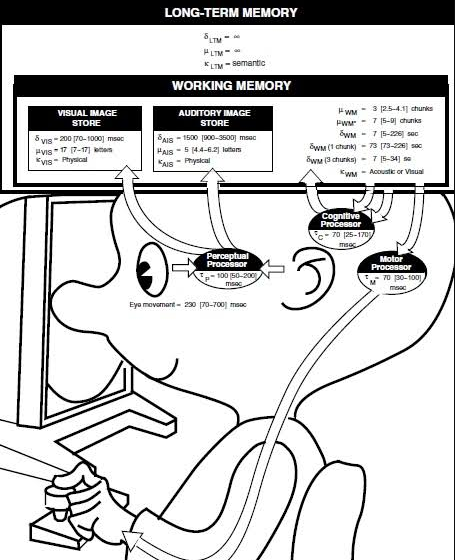
\includegraphics[width=0.3\linewidth]{image/hip}
%	\end{figure}
\end{frame}



%\begin{frame}
%\frametitle{Vision}
%\begin{itemize}
%	\item Seeing begins with the reception of light through the eye's lens, then the lens focuses the light into an image projected on to the retina, the retina then convert light into neurological signal sent to the brain via optic nerve
%	\begin{figure}
%		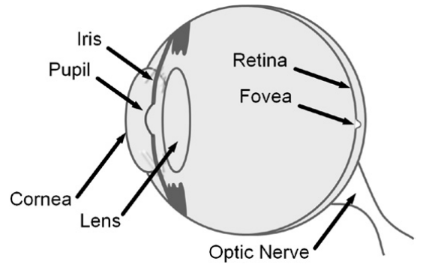
\includegraphics[width=0.6\linewidth]{image/eye}
%		\caption{Source: Fg 2.3 (Mackenzie)}
%	\end{figure}
%\end{itemize}
%\end{frame}

\section{Perception}

\begin{frame}
	\frametitle{Perception}
	\begin{itemize}
		\item \textbf{First stage of processing} in the brain, occurs when sensory signals are received as input.  It is at this stage human makes meanings
		\item Perception has been studied in a area of experimental psychology known as \textbf{psychophysics} - examines the relationship between perception and physical phenomena
%		\item In psychophysics experiment, human is presented with physical stimulus and is then asked how they felt/perceive
%		\item A common experimental goal is to measure \textit{just noticeable difference} (JND) - does the two stimuli differ?  By manipulating the small difference between two stimuli, we can better understand human perception 
	\end{itemize}
\end{frame}

\begin{frame}
\frametitle{Facts about Perception}
\begin{enumerate}
	\item Our perception is biased by
	\begin{itemize}
		\item our goals
		\item our belief
		\item our experience
		\item the context
	\end{itemize}
	\item Our vision is optimized to see structure
	\item Our color vision is limited
	\item Our peripheral vision is poor
	\item Visual search is linear unless target "pops"
	\item Reading is unnatural
\end{enumerate}
\end{frame}

\subsection{Biases}

\begin{frame}
\frametitle{Our perception is biased...}
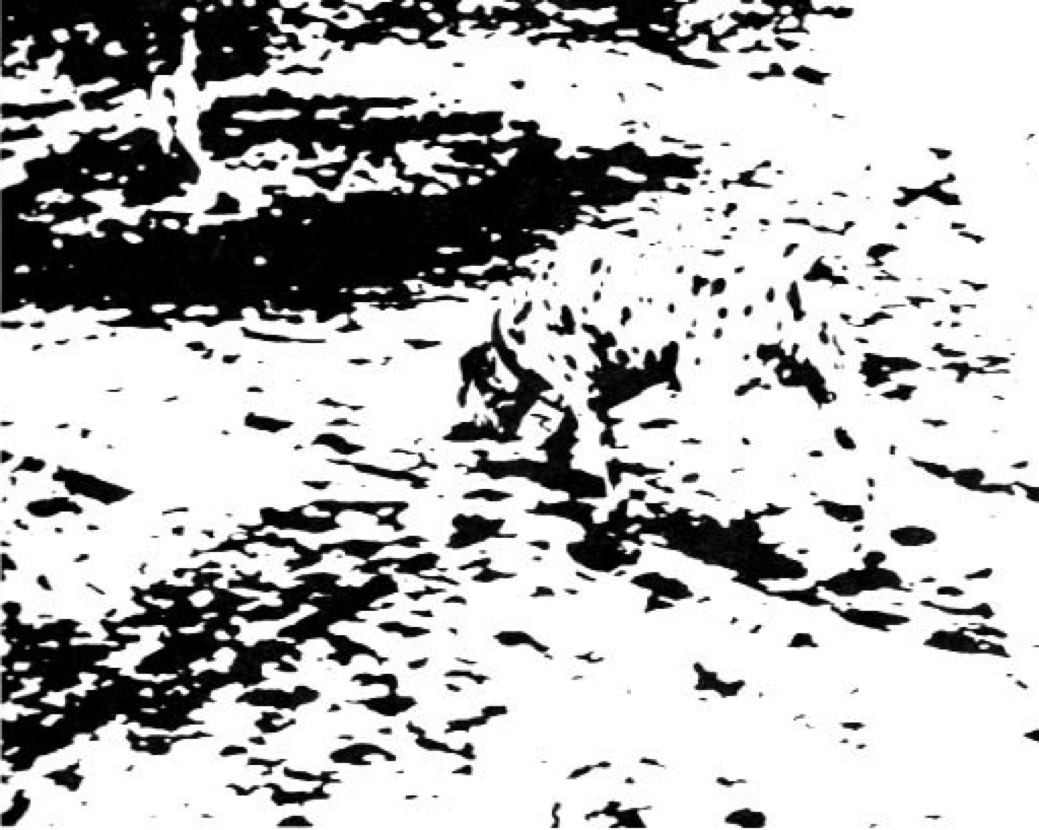
\includegraphics[width=0.8\linewidth]{image/perception1}
\end{frame}

\begin{frame}
\frametitle{Our perception is biased...}
\centering
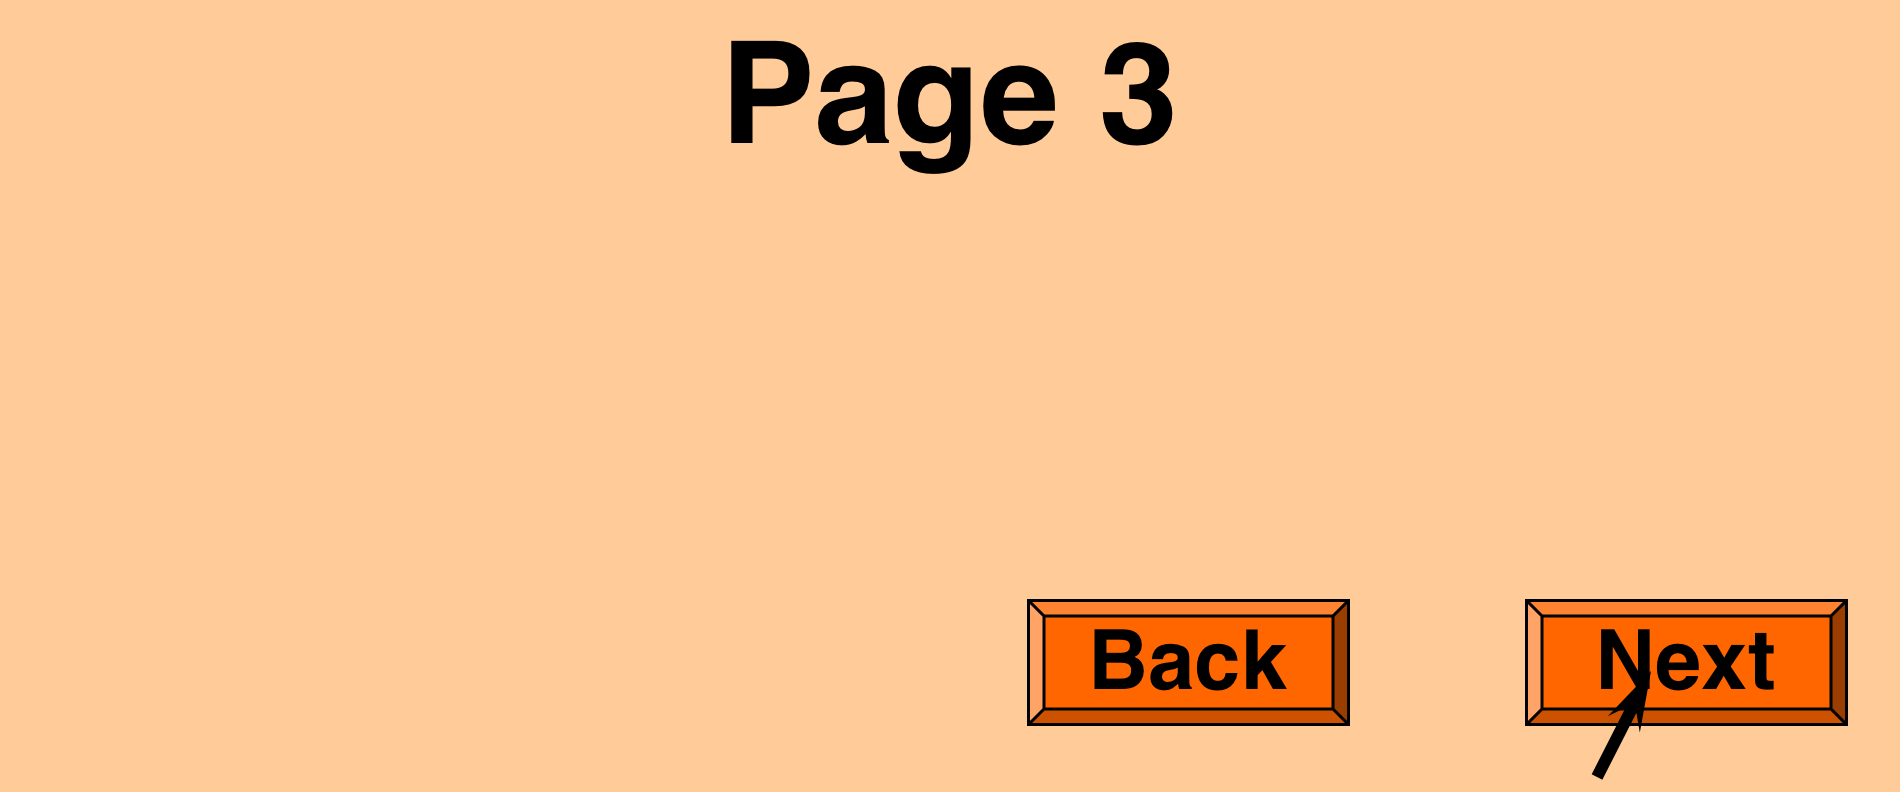
\includegraphics[width=0.6\linewidth]{image/perception3}
\vfill
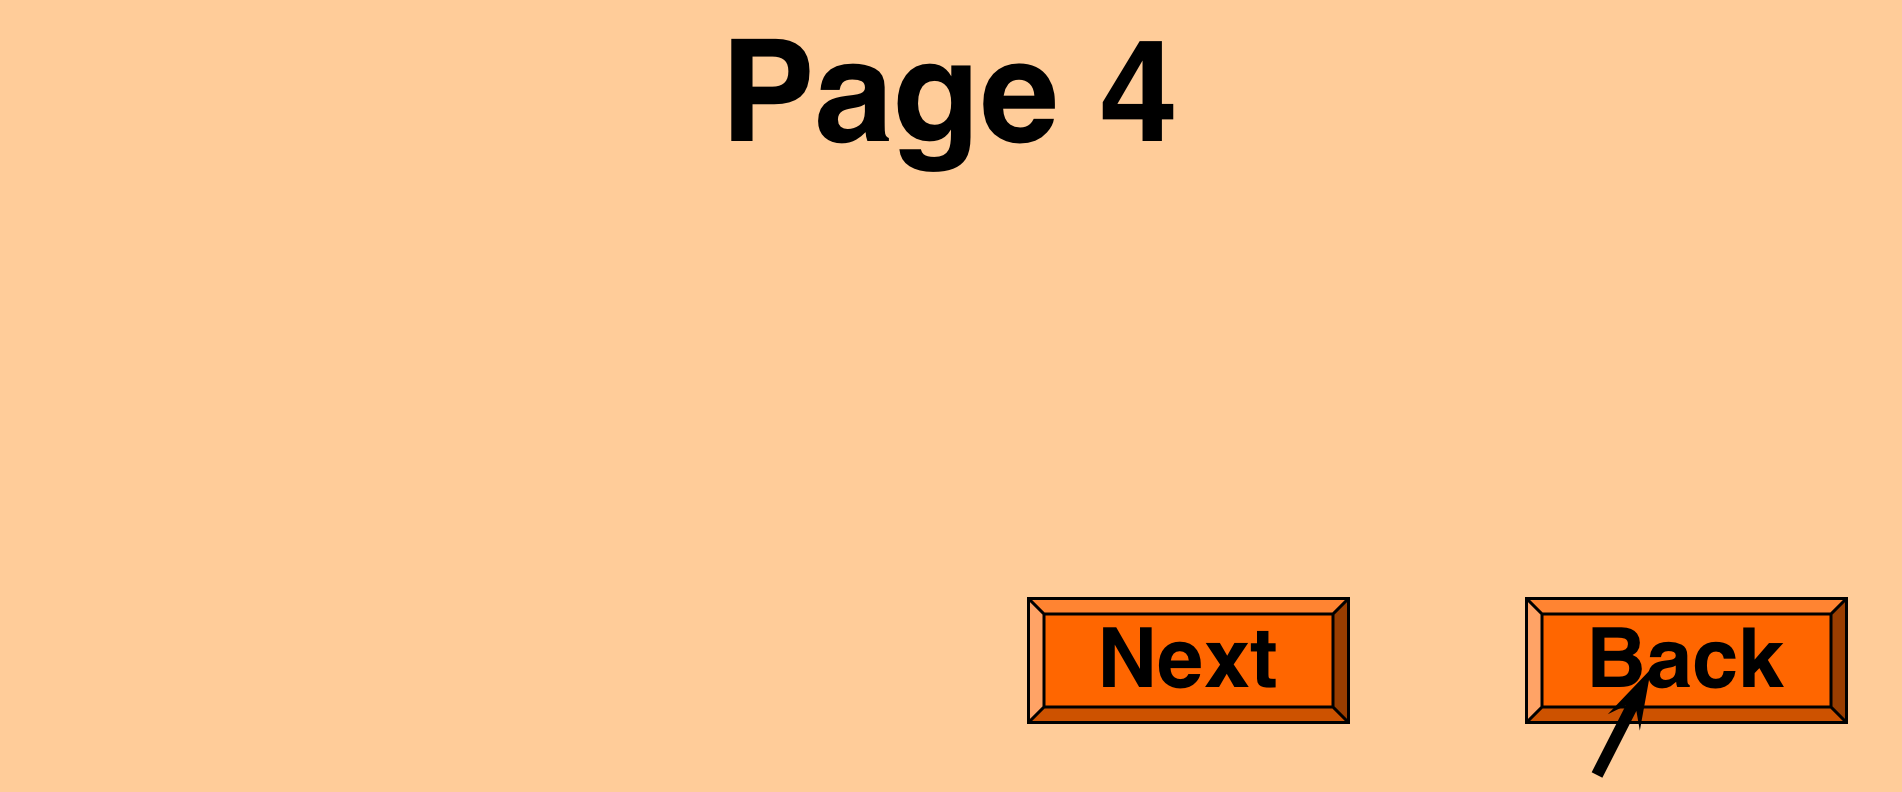
\includegraphics[width=0.6\linewidth]{image/perception2}
\end{frame}

\begin{frame}
\frametitle{Our perception is biased...}
Exactly same character
\centering

\includegraphics[width=0.8\linewidth]{image/perception4}
\end{frame}

\begin{frame}
\frametitle{Our perception is biased...}
But our perception can be changed based on the \textbf{context}
\centering

\includegraphics[width=0.8\linewidth]{image/perception5}
\end{frame}

\begin{frame}
\frametitle{Our perception is biased...}
Muller-Lyer illusion 
\centering
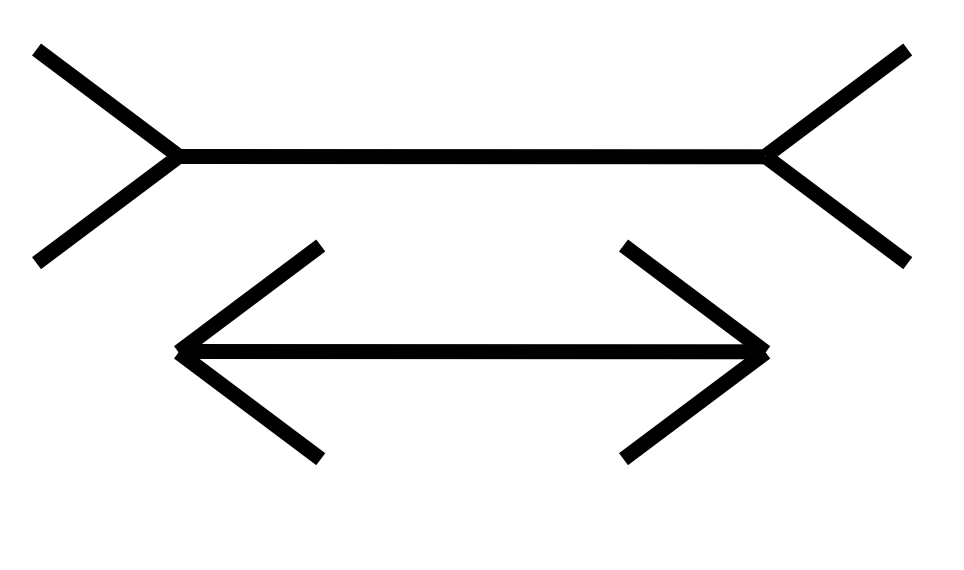
\includegraphics[width=0.8\linewidth]{image/perception8}
\end{frame}

\begin{frame}
\frametitle{Our perception is biased...}
Muller-Lyer illusion 
\centering
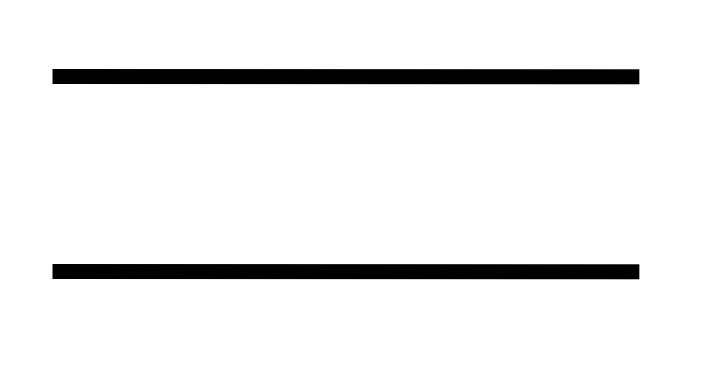
\includegraphics[width=0.8\linewidth]{image/perception7}
\end{frame}

\begin{frame}
\frametitle{Our perception is biased...}
All lines in this image are straight!
\centering
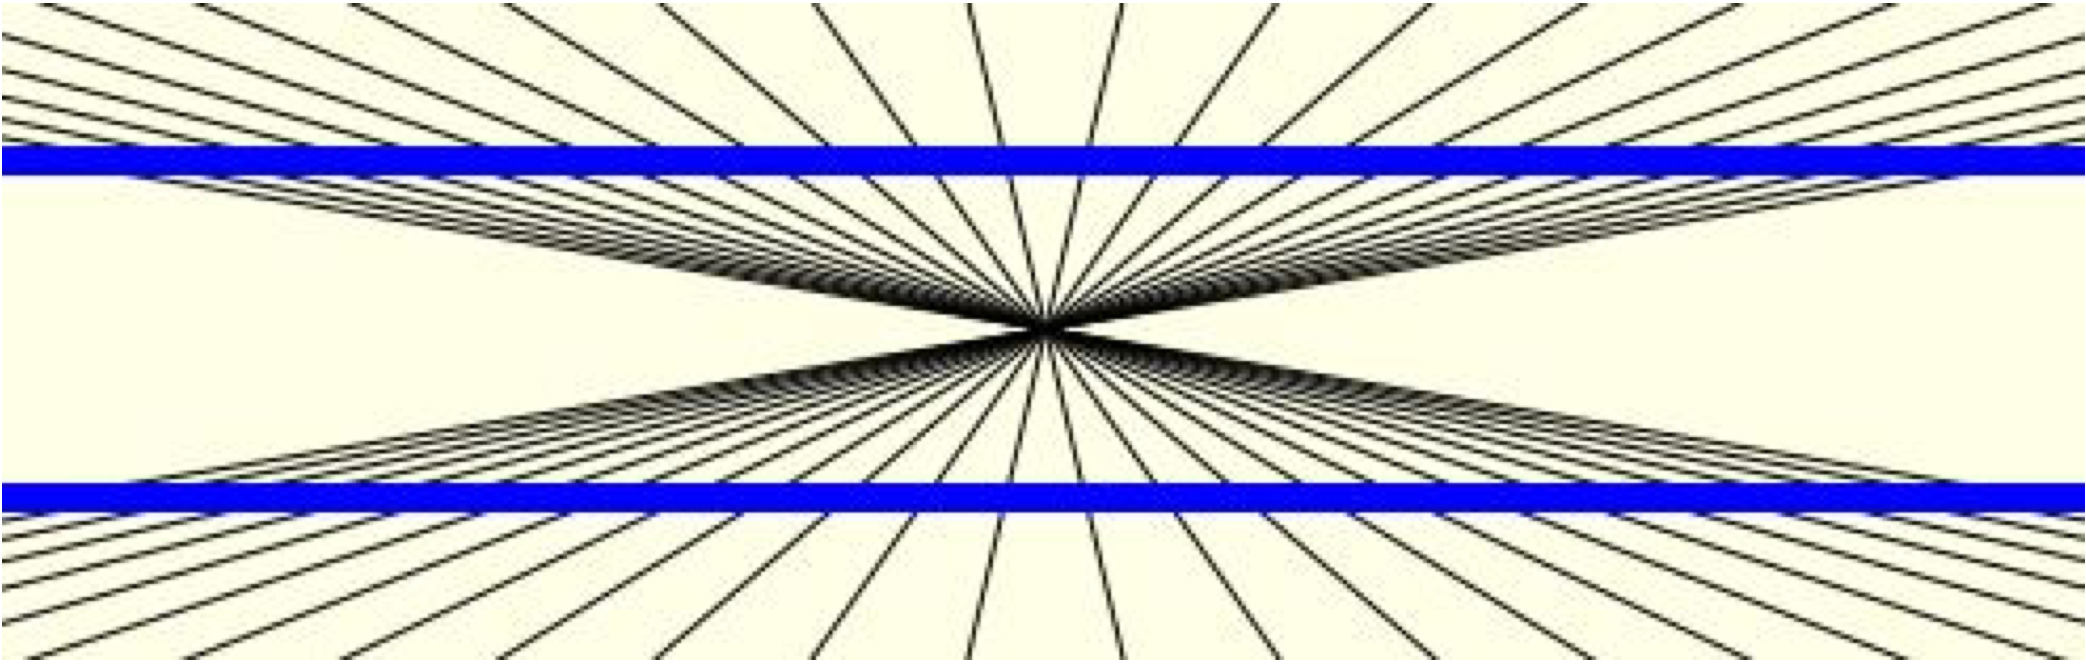
\includegraphics[width=1\linewidth]{image/perception9}
\end{frame}

\begin{frame}
\frametitle{Our perception is biased...}
Gray lines are straight, horizontal, and parallel!
\centering

\includegraphics[width=1\linewidth]{image/perception10}
\end{frame}

\begin{frame}
\frametitle{Our perception is biased by goals}
\begin{itemize}
\item Our perception is biased toward our \textbf{goals}
\item Tend not to notice things unrelated to goals
\end{itemize}
\end{frame}

\begin{frame}
\frametitle{Our perception is biased by goals}
\centering
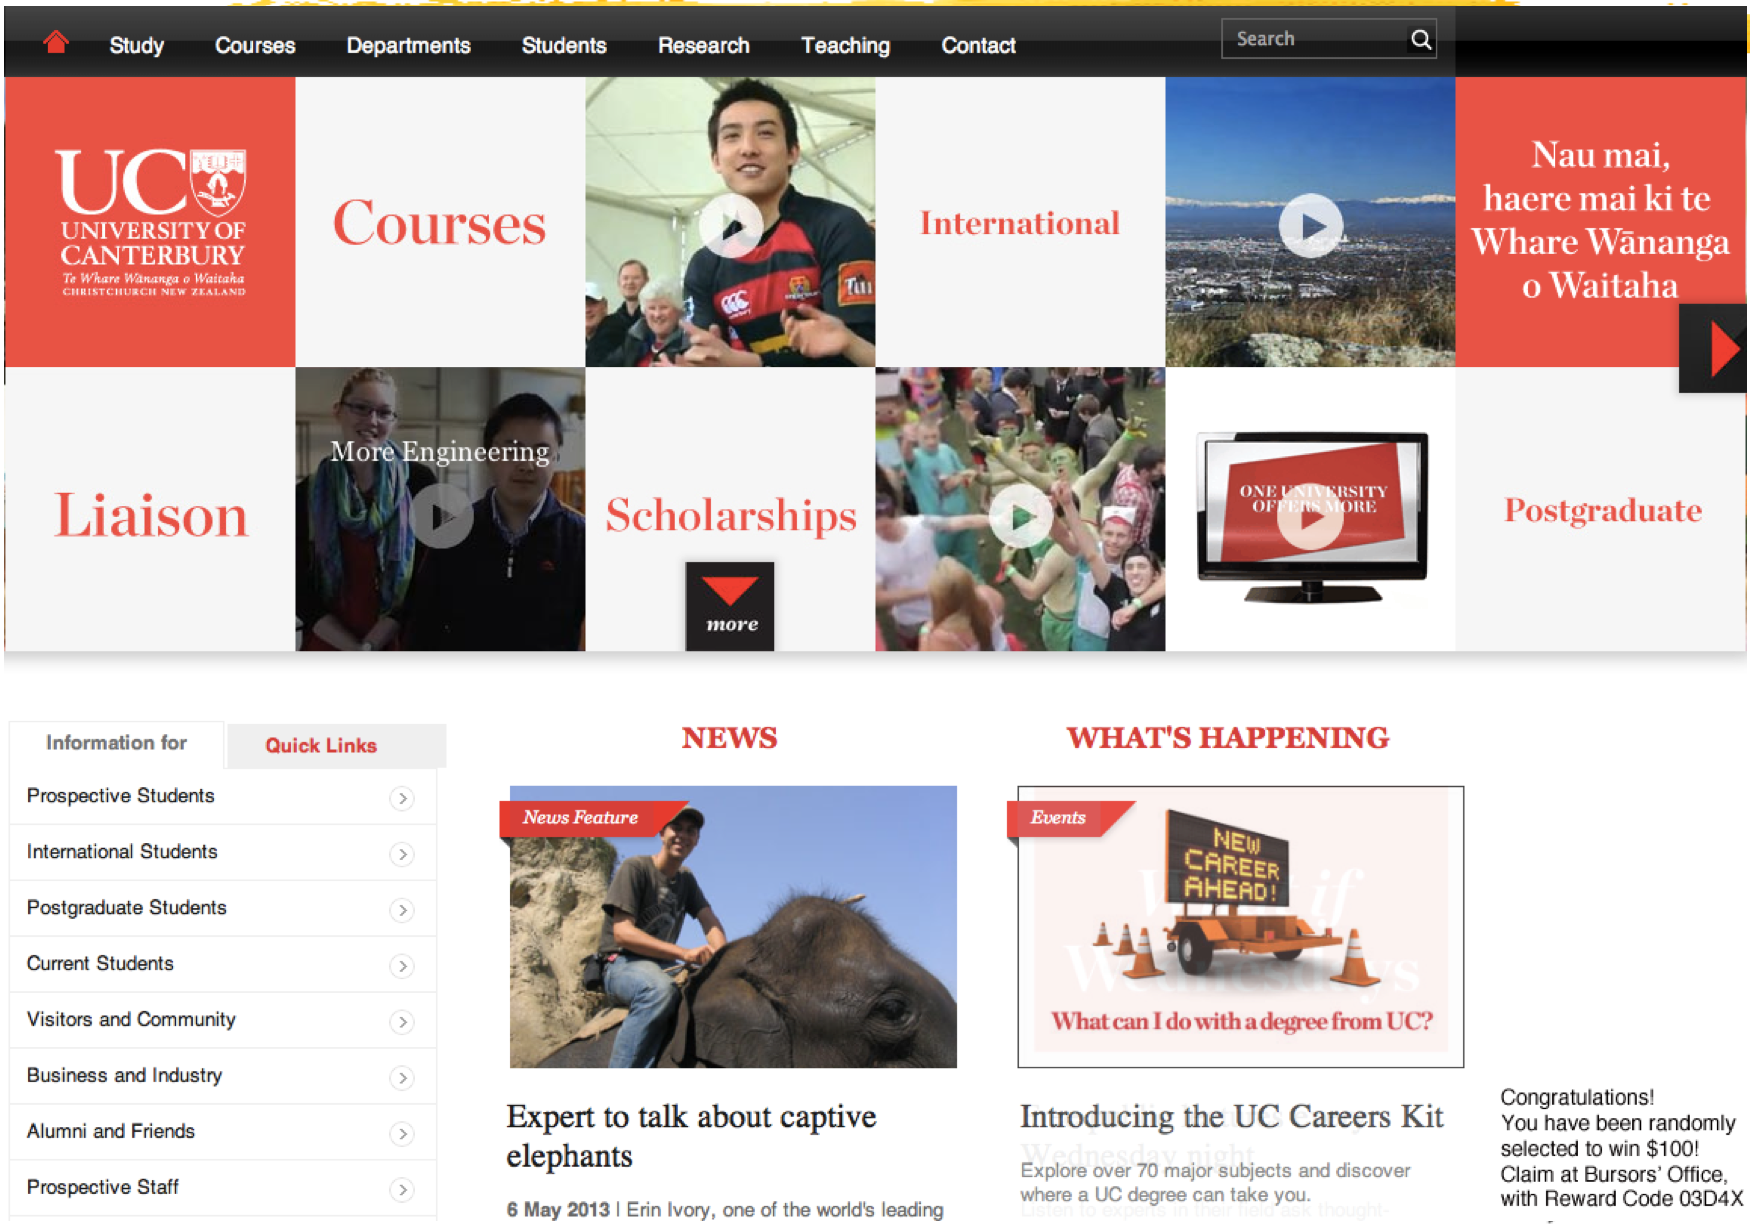
\includegraphics[width=0.8\linewidth]{image/perception11}
\end{frame}

\begin{frame}
\frametitle{Our perception is biased by goals}
\centering
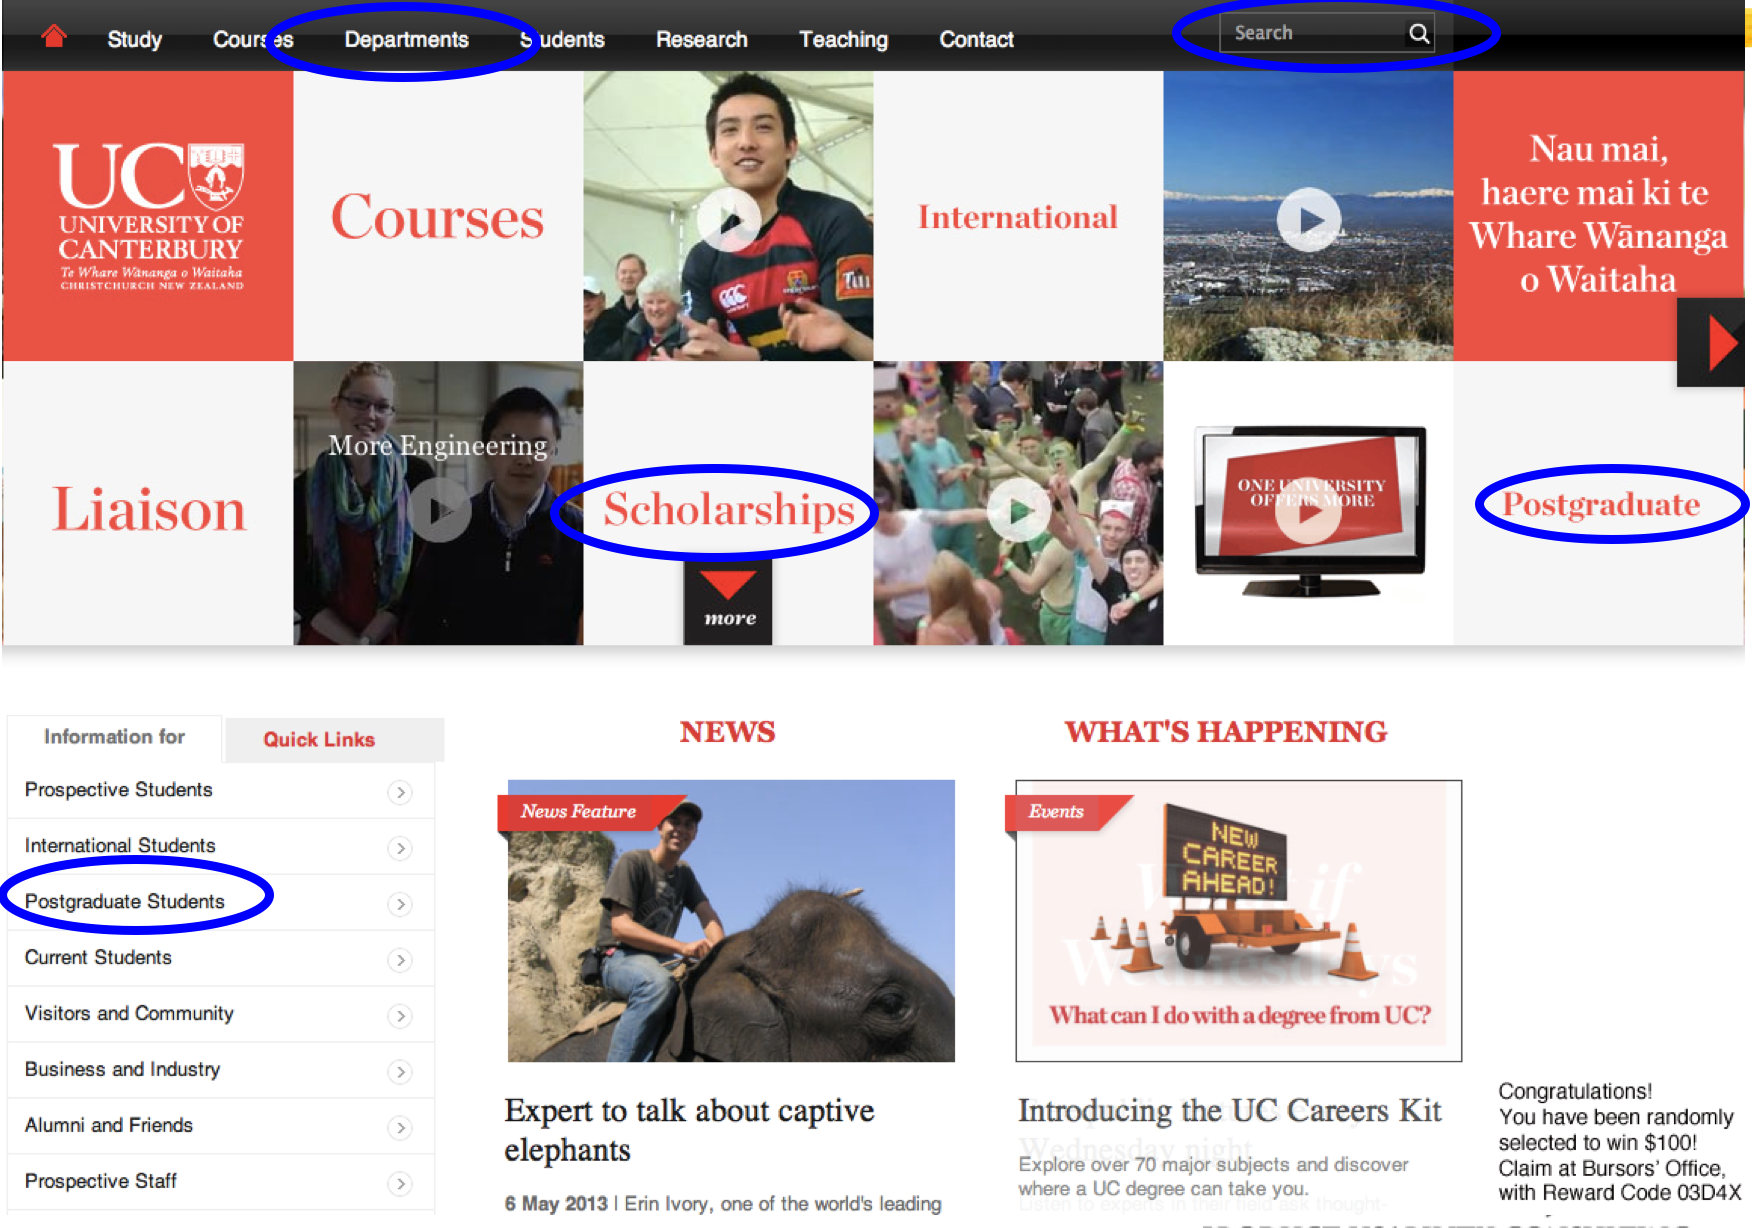
\includegraphics[width=0.8\linewidth]{image/perception12}
\end{frame}

\subsection{Structure}

\begin{frame}
\frametitle{Our vision is optimized to see structures}
Gestalt Principles of Visual Perception
\begin{itemize}
\item Proximity
\item Similarity
\item Continuity
\item Closure
\item Symmetry
\item Figure/ground
\item Common fate
\end{itemize}
\end{frame}

%\begin{frame}
%\frametitle{Gestalt}
%\centering
%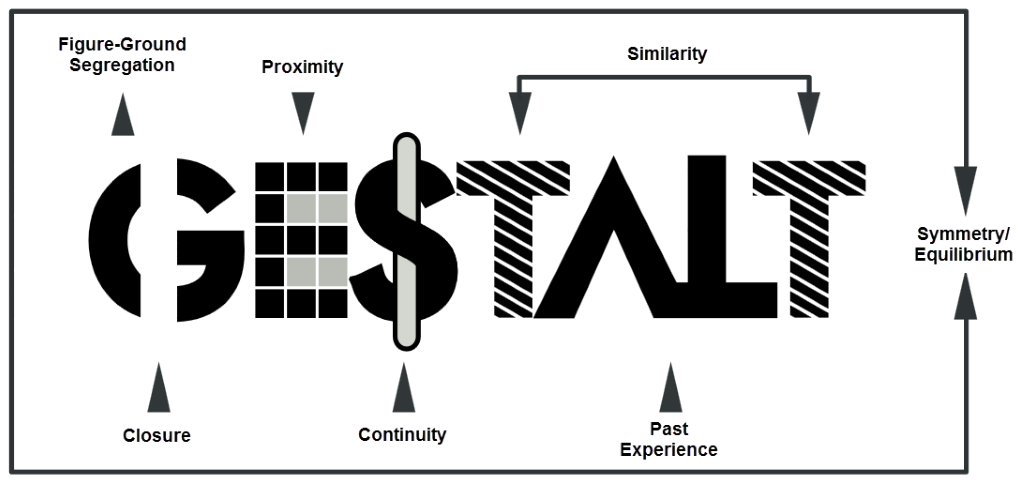
\includegraphics[width=1\linewidth]{image/gestalt}
%\end{frame}

\begin{frame}
\frametitle{Proximity}
\centering
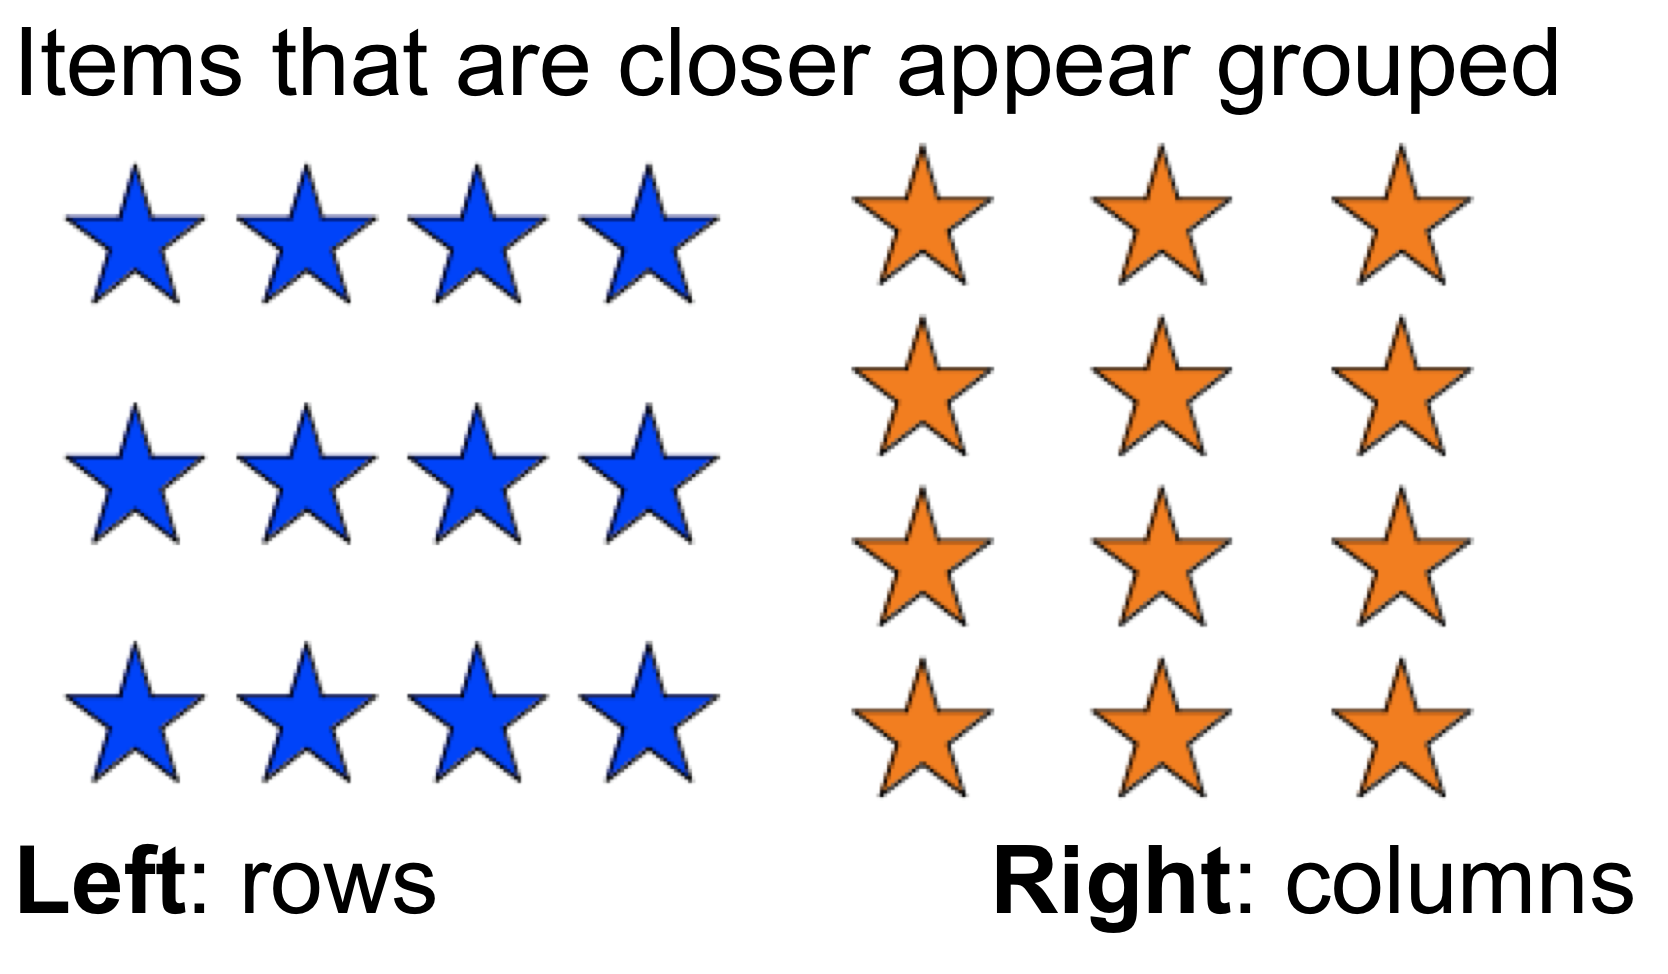
\includegraphics[width=0.8\linewidth]{image/proximity}
\end{frame}

\begin{frame}
\frametitle{Proximity}
\centering
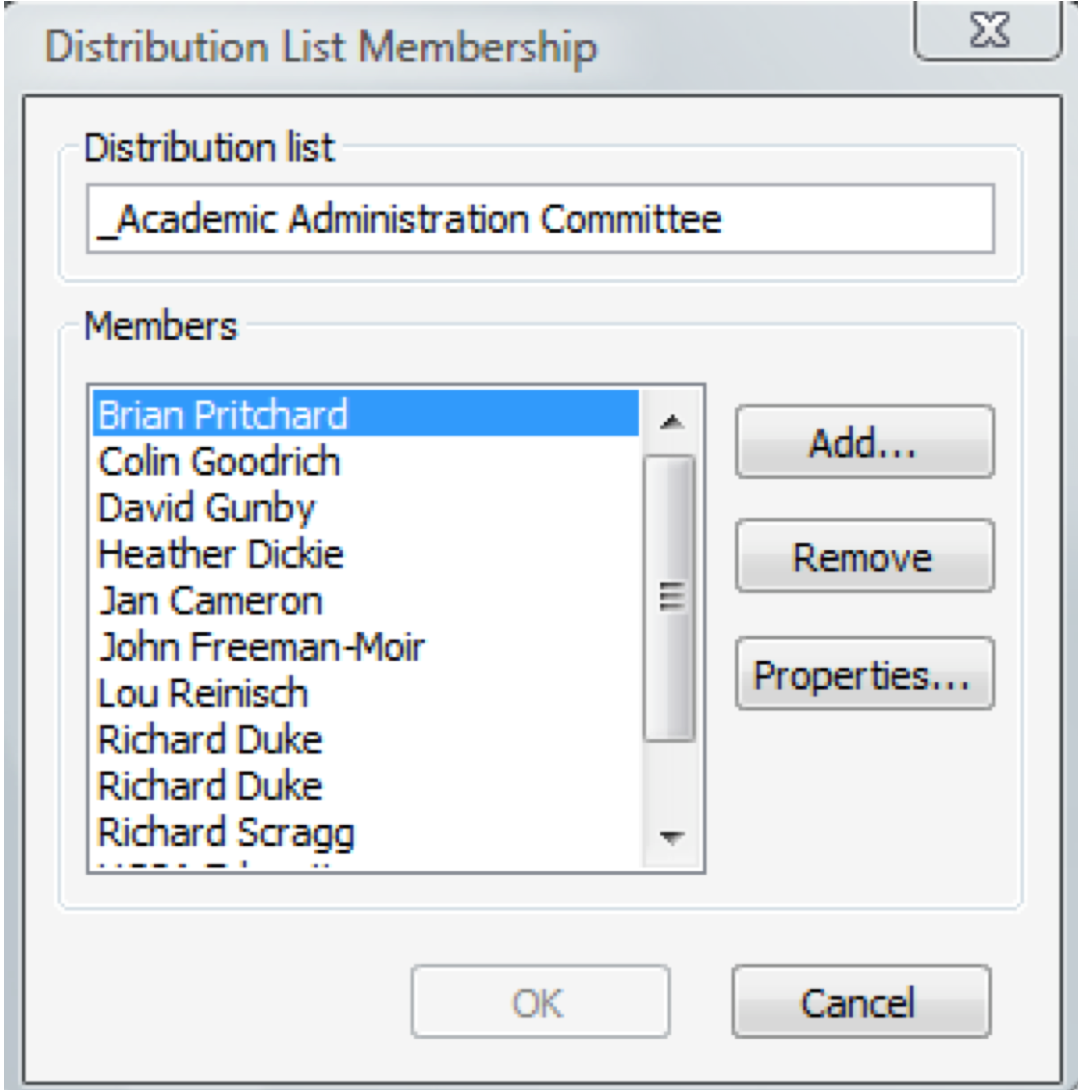
\includegraphics[width=0.5\linewidth]{image/proximity2}
\end{frame}

\begin{frame}
\frametitle{Proximity}
\centering
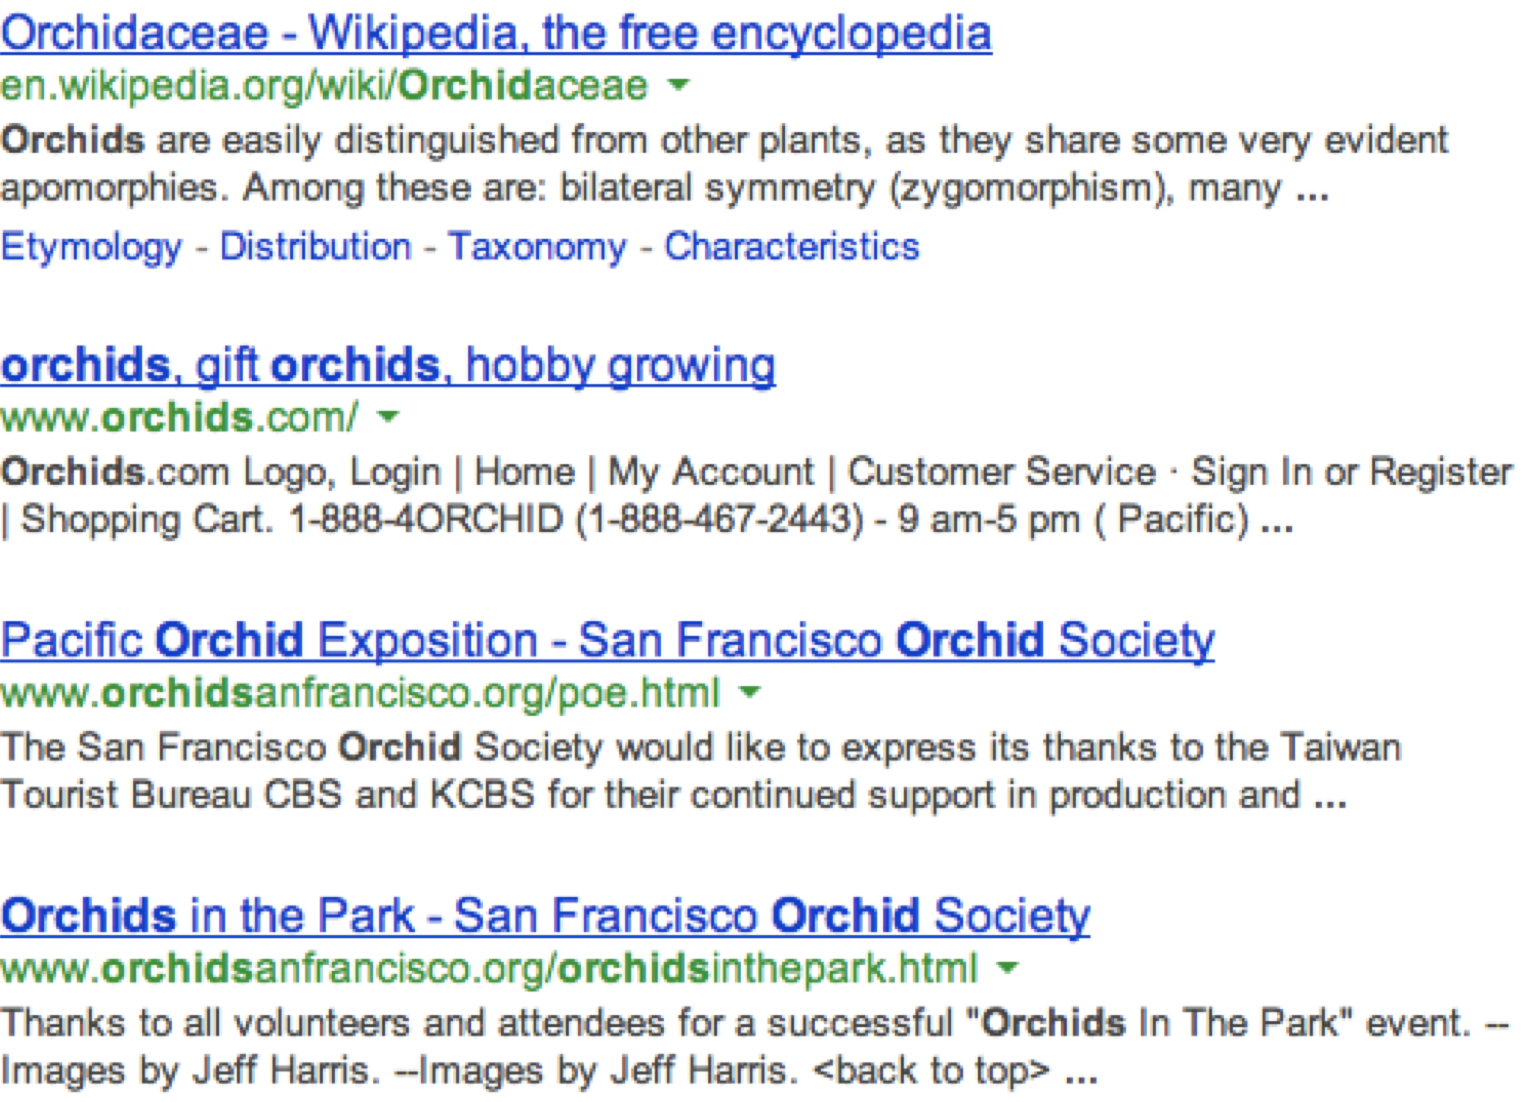
\includegraphics[width=0.8\linewidth]{image/proximity3}
\end{frame}

\begin{frame}
	\frametitle{Proximity}
	\centering
	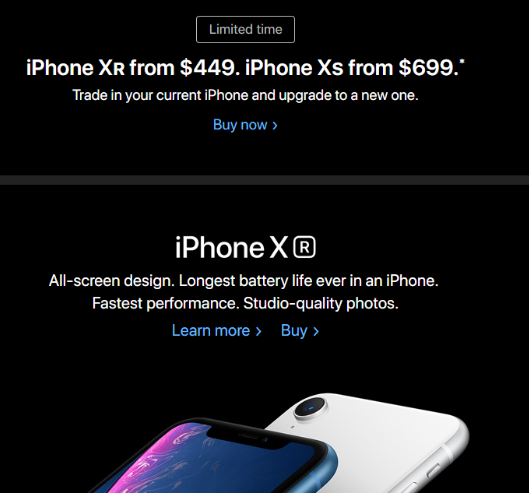
\includegraphics[width=0.6\linewidth]{image/proximity4}
\end{frame}

\begin{frame}
\frametitle{Closure}
We tend to see whole, closed objects, not collections of fragments \newline
\centering
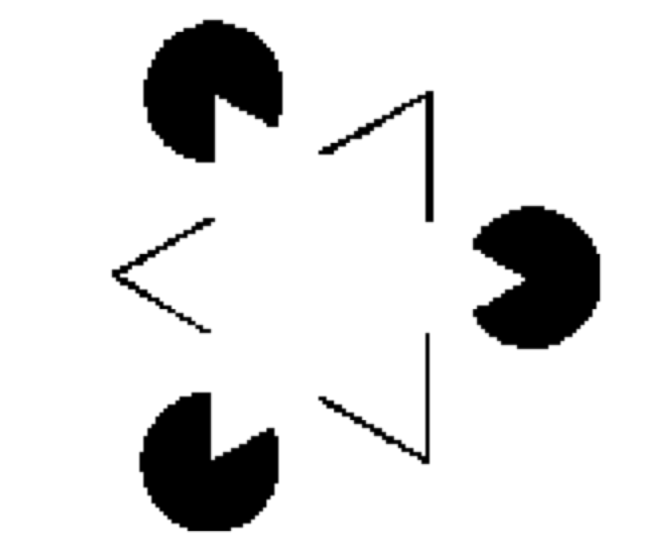
\includegraphics[width=0.5\linewidth]{image/closure}
\end{frame}

\begin{frame}
\frametitle{Closure}
We tend to see whole, closed objects, not collections of fragments \newline
\centering
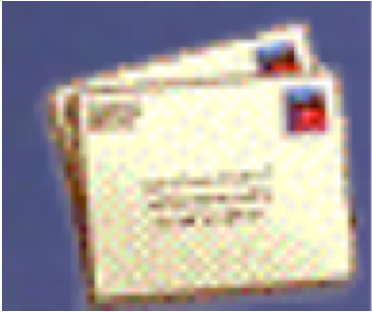
\includegraphics[width=0.3\linewidth]{image/closure2}
\end{frame}

\begin{frame}
\frametitle{Simplicity}
We tend to see simple figures rather than complex ones
\centering

\includegraphics[width=0.5\linewidth]{image/symmetry}
\end{frame}

\begin{frame}
\frametitle{Figure/Ground}
The tendency to simplify based on the figures and the grounds

\centering
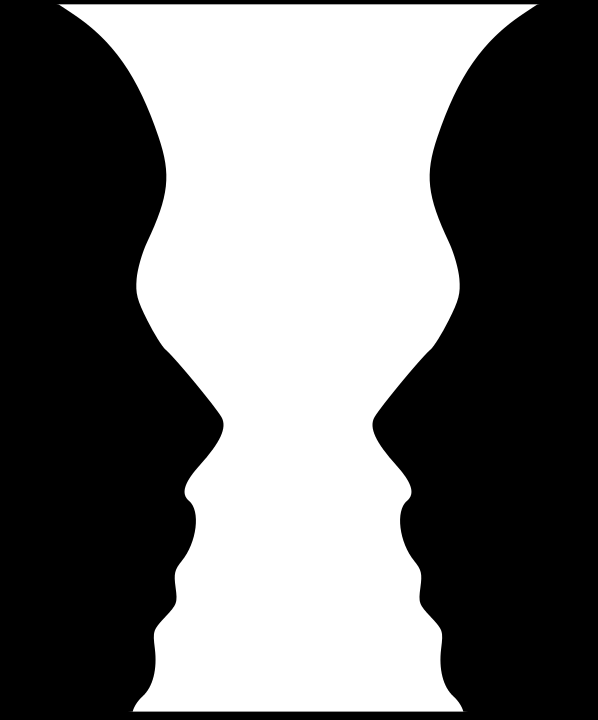
\includegraphics[width=0.4\linewidth]{image/ground}
\end{frame}

%\begin{frame}
%\frametitle{We seek and use visual structure}
%\centering
%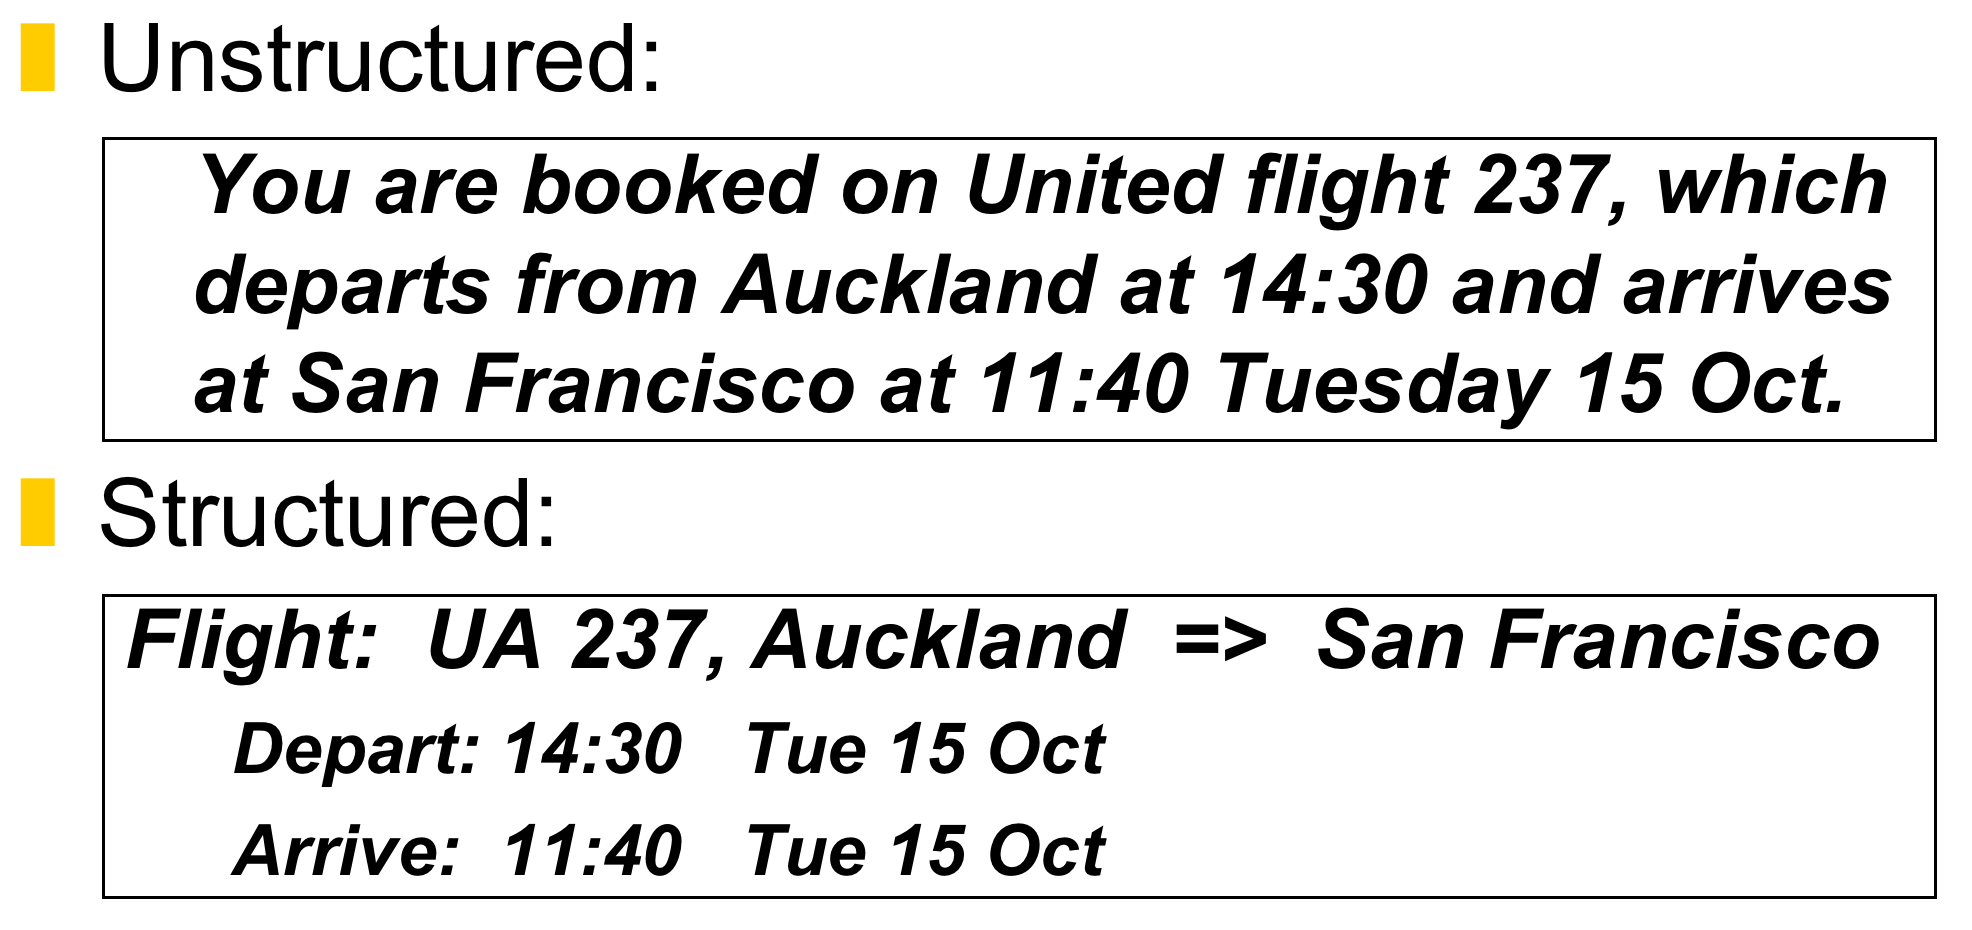
\includegraphics[width=1\linewidth]{image/structure}
%\end{frame}
%
%\begin{frame}
%\frametitle{We seek and use visual structure}
%Human loves hierarchy...for some reasons...
%\centering
%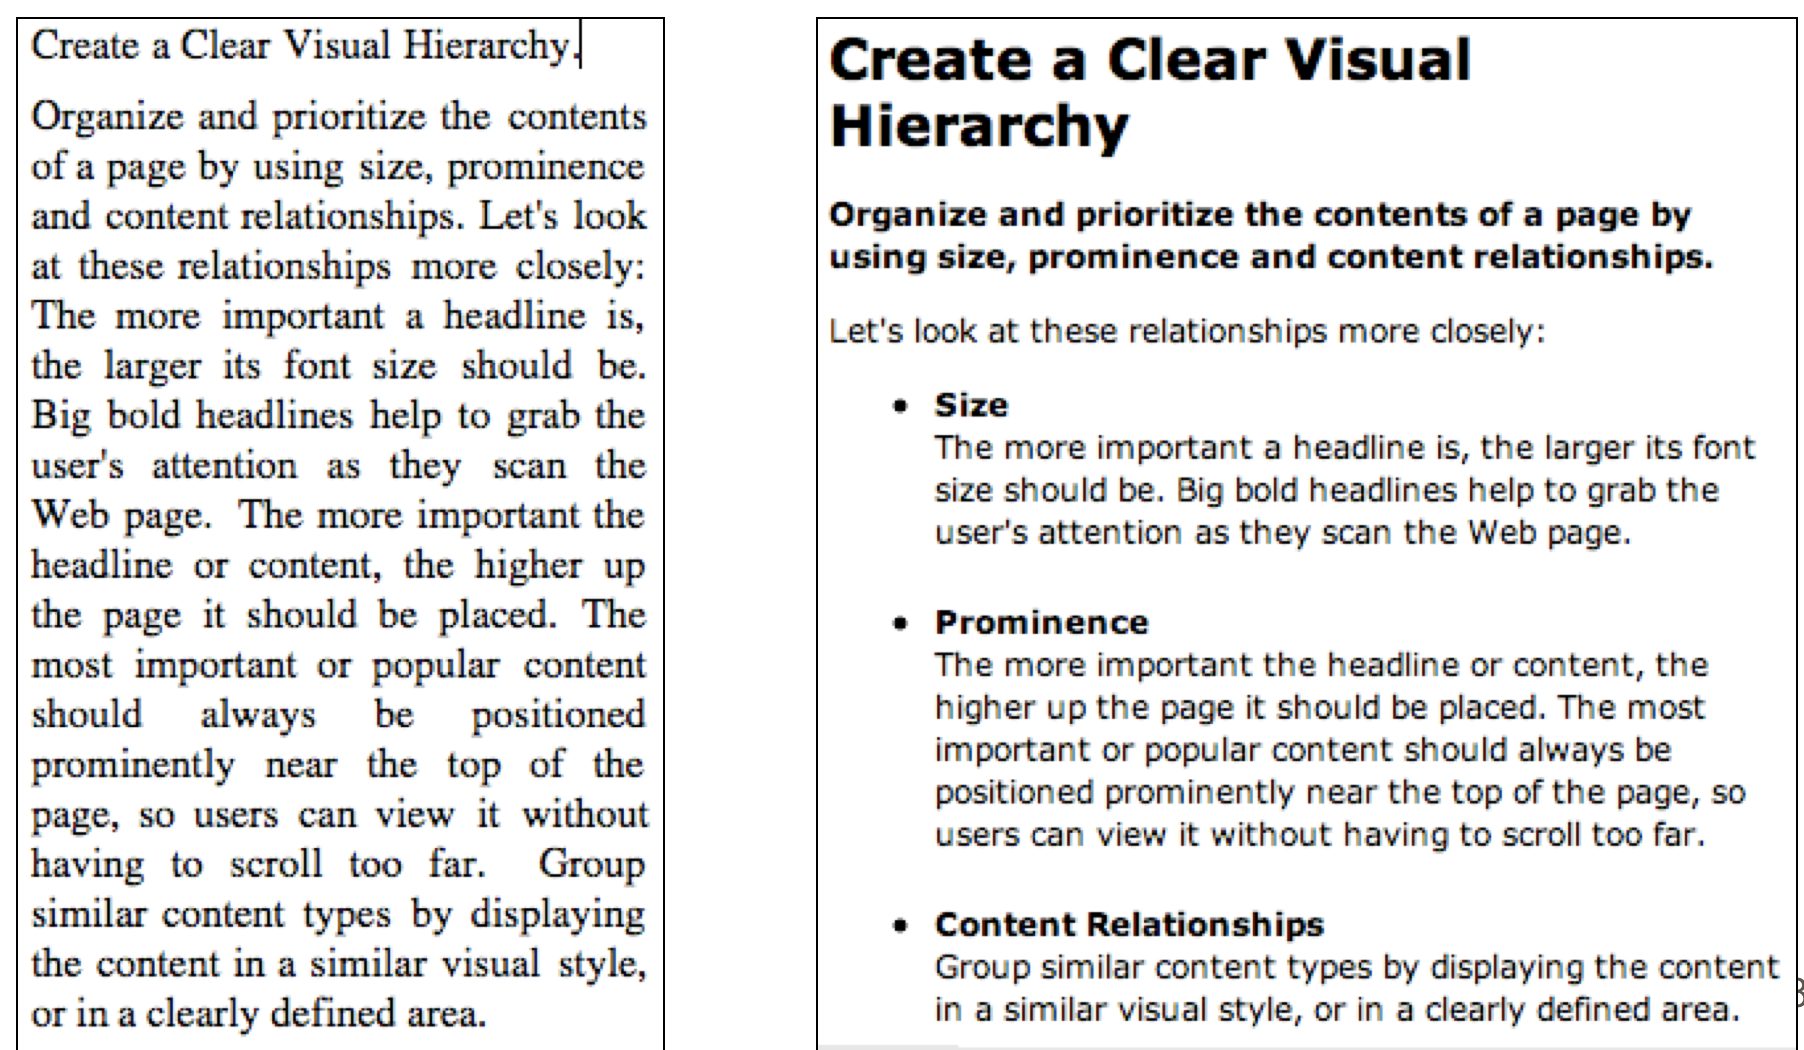
\includegraphics[width=1\linewidth]{image/structure2}
%\end{frame}
%
%\begin{frame}
%\frametitle{We seek and use visual structure}
%Structured numbers are easier to see...
%\centering
%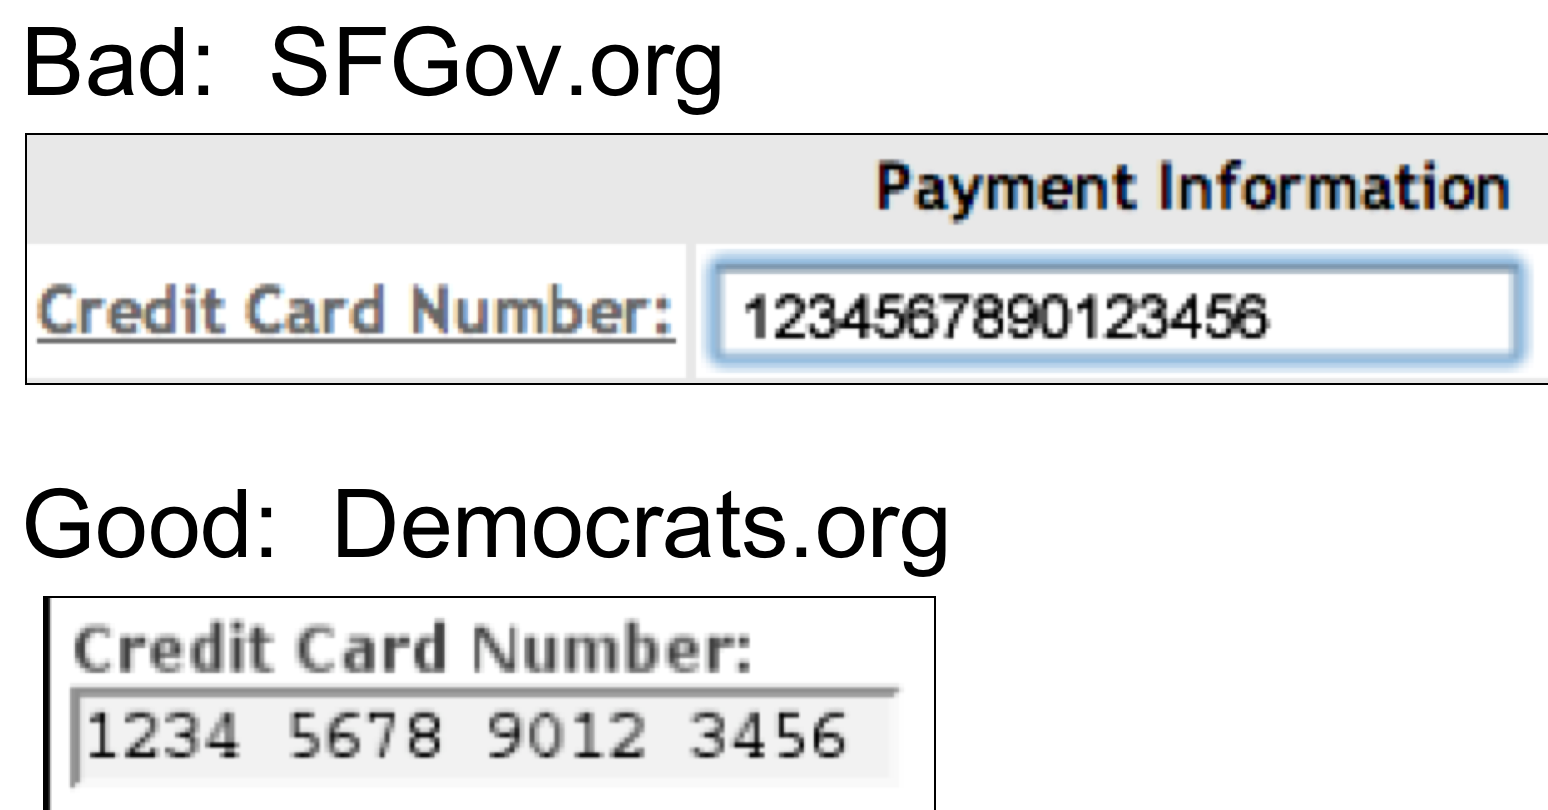
\includegraphics[width=1\linewidth]{image/structure3}
%\end{frame}

\subsection{Limitations}

\begin{frame}
\frametitle{Our color vision is limited...}
Optimized to see contrasts, edges, and changes, not absolute levels
\centering
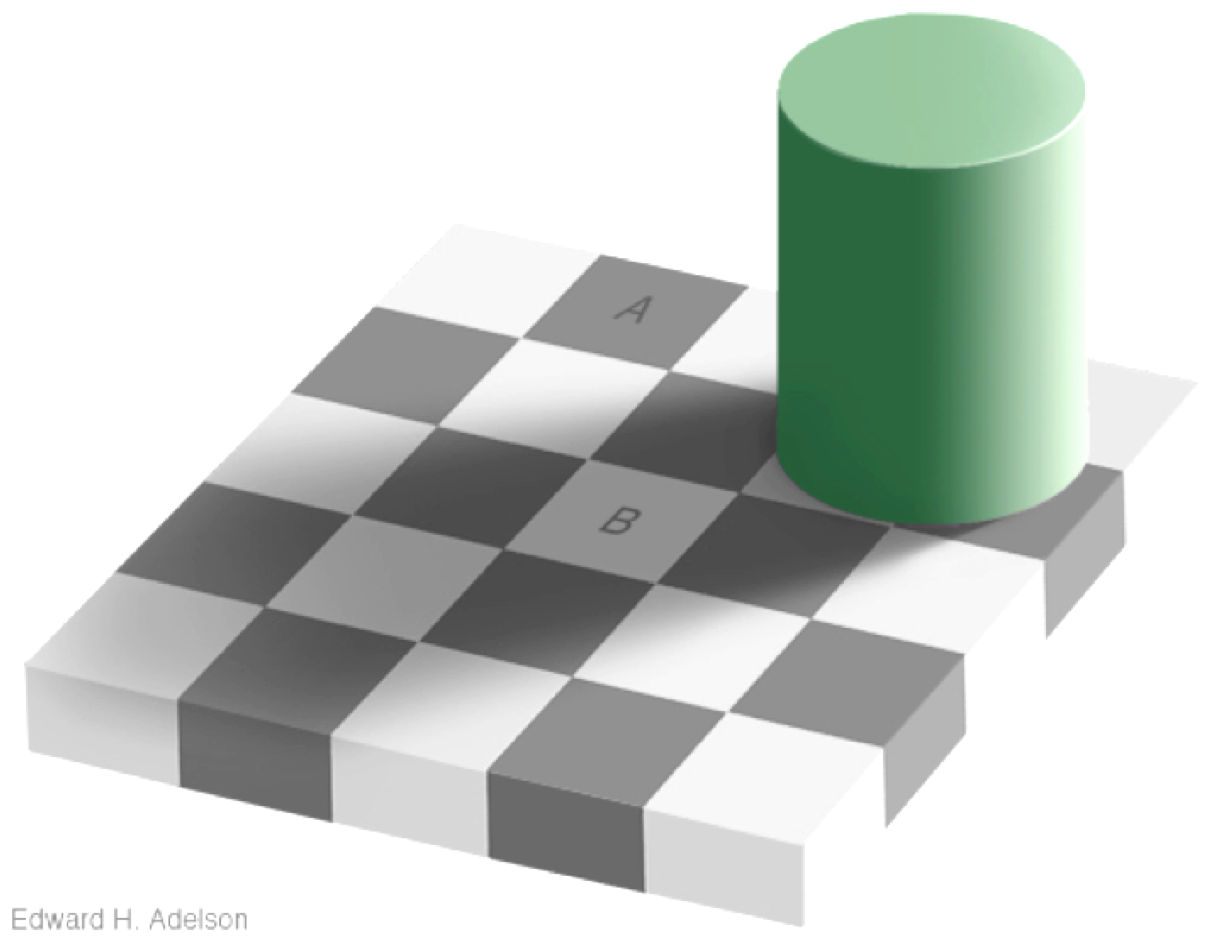
\includegraphics[width=0.6\linewidth]{image/vision}
\end{frame}

\begin{frame}
\frametitle{Our color vision is limited...}
Optimized to see contrasts, edges, and changes, not absolute levels
\centering
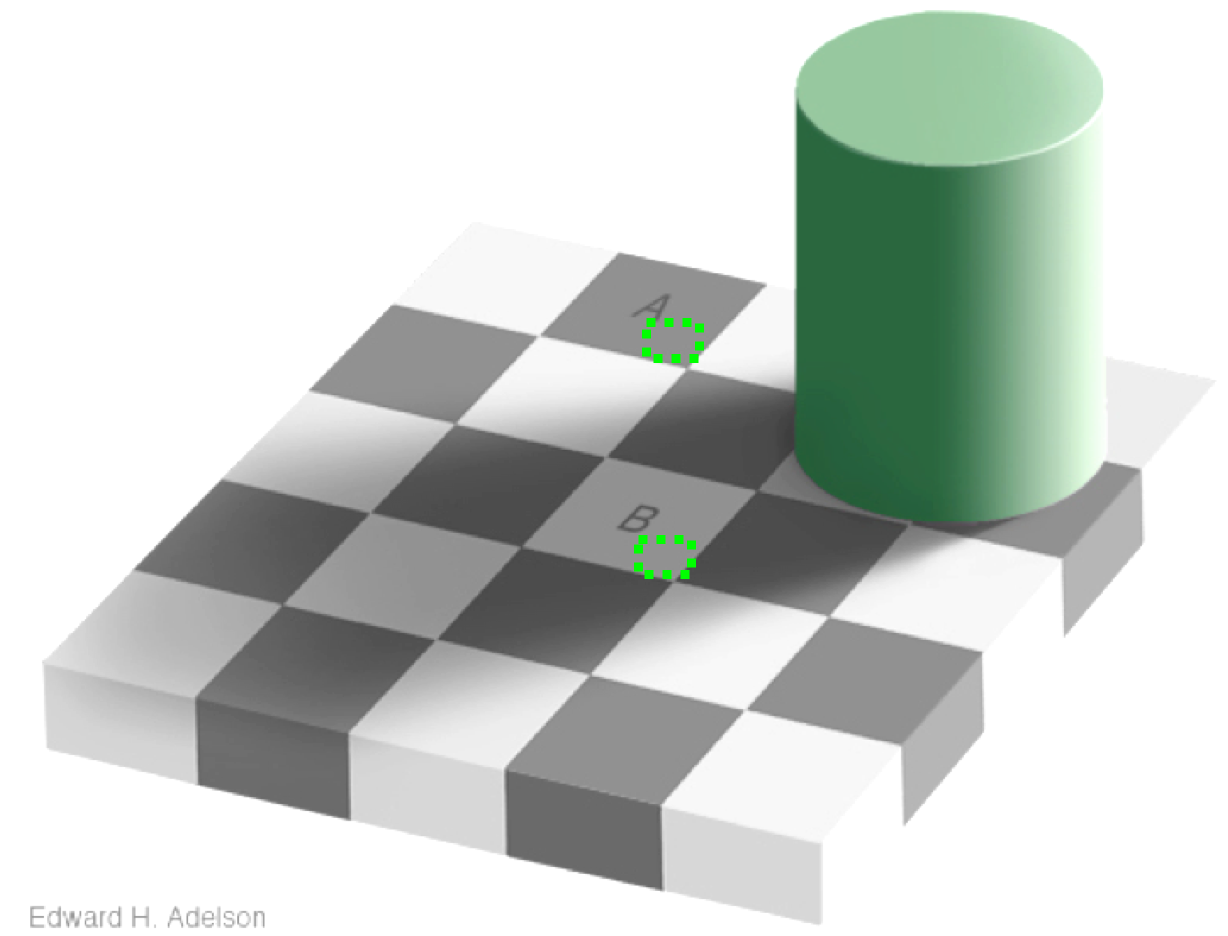
\includegraphics[width=0.6\linewidth]{image/vision2}
\end{frame}

\begin{frame}
\frametitle{Our color vision is limited...}
Optimized to see contrasts, edges, and changes, not absolute levels
\centering
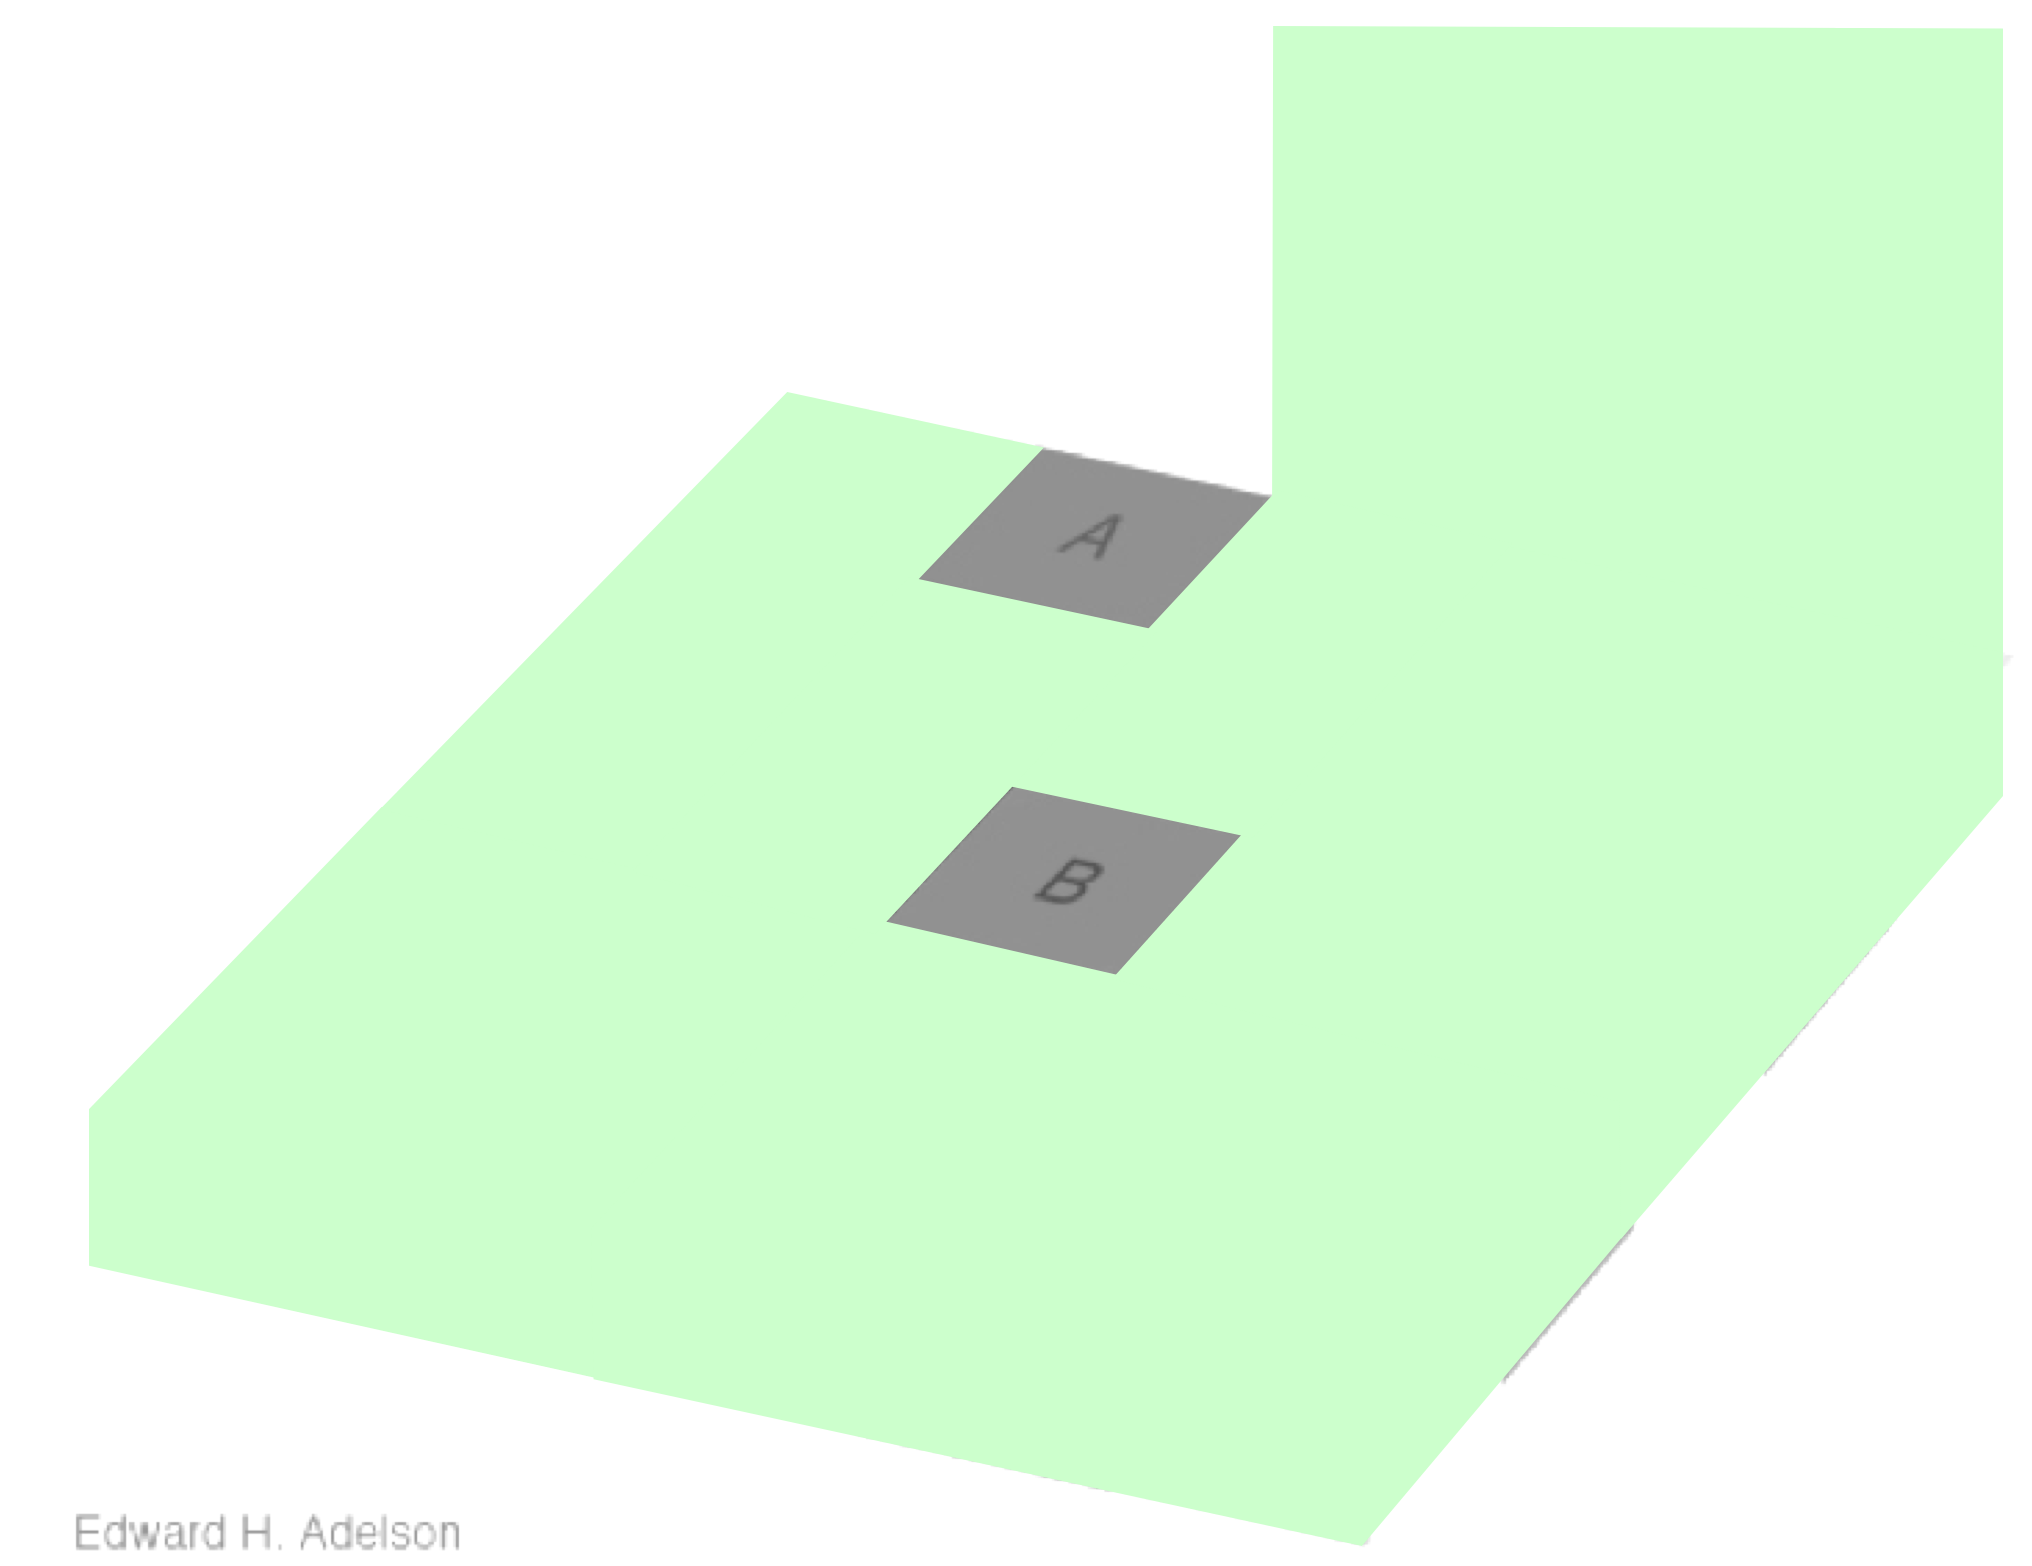
\includegraphics[width=0.6\linewidth]{image/vision3}
\end{frame}

\begin{frame}
\frametitle{Our color vision is limited...}
We have trouble discriminating - pale colors, small color patches, separated patches...
\vfill
\centering
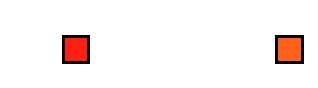
\includegraphics[width=0.2\linewidth]{image/vision4}
\end{frame}

\begin{frame}
\frametitle{Our color vision is limited...}
We have trouble discriminating - pale colors, small color patches, separated patches...
\vfill
\centering
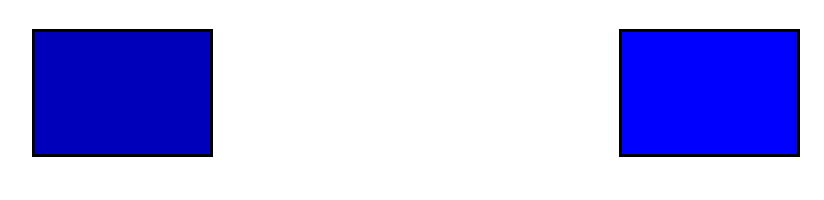
\includegraphics[width=0.5\linewidth]{image/vision5}
\end{frame}

\begin{frame}
\frametitle{Our color vision is limited...}
We have trouble discriminating - pale colors, small color patches, separated patches...
\vfill
\centering
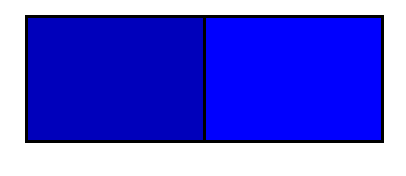
\includegraphics[width=0.3\linewidth]{image/vision6}
\end{frame}

\begin{frame}
\frametitle{Our color vision is limited...}
Some people have color blindness
\begin{itemize}
\item ~ 8\% of males
\item ~ 0.5\% of females
\end{itemize}
\vfill
\centering
colors that would be hard for red-green colorblind people to distinguish \vfill
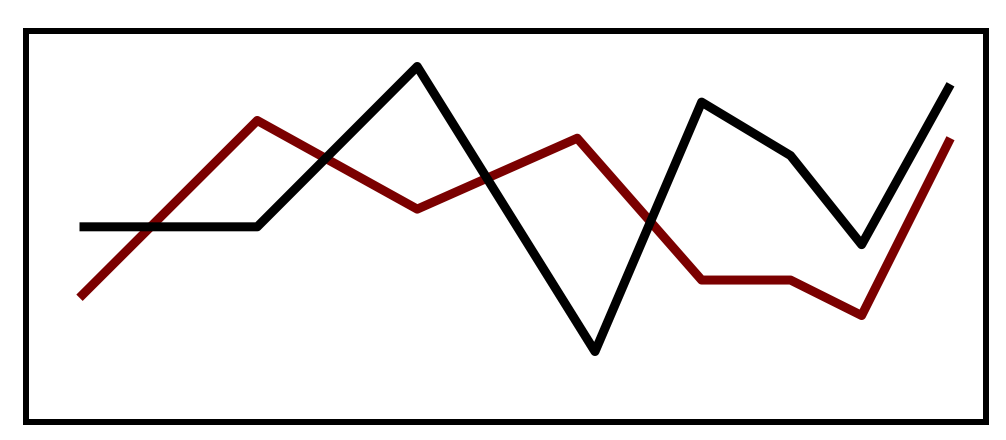
\includegraphics[width=0.8\linewidth]{image/colorblind}
\end{frame}

\begin{frame}
\frametitle{Our color vision is limited...}
Most common forms of color blindness - red-green called deuteranopia
\vfill
\centering
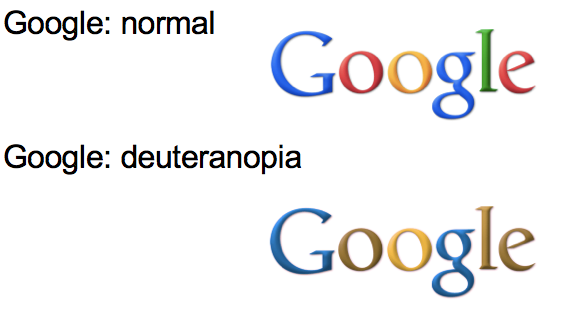
\includegraphics[width=0.8\linewidth]{image/colorblind2}
\end{frame}

\begin{frame}
\frametitle{Our color vision is limited...}
Don't use colors only!  Also rely on other things like shapes or cues
\vfill
\centering
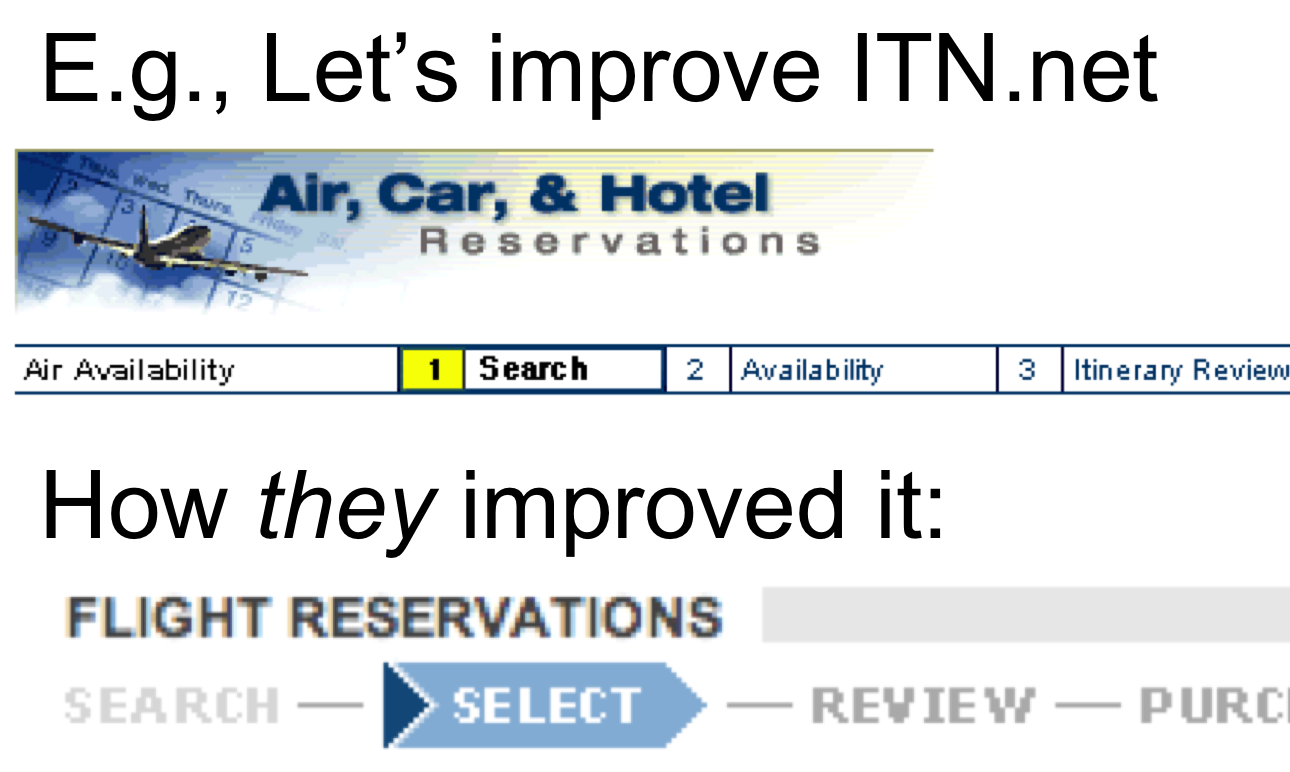
\includegraphics[width=0.8\linewidth]{image/colorblind3}
\end{frame}

\begin{frame}
\frametitle{Our color vision is limited...}
Don't use subtle color differences.  Should still look different in gray scales.  Bad examples below....
\vfill
\centering
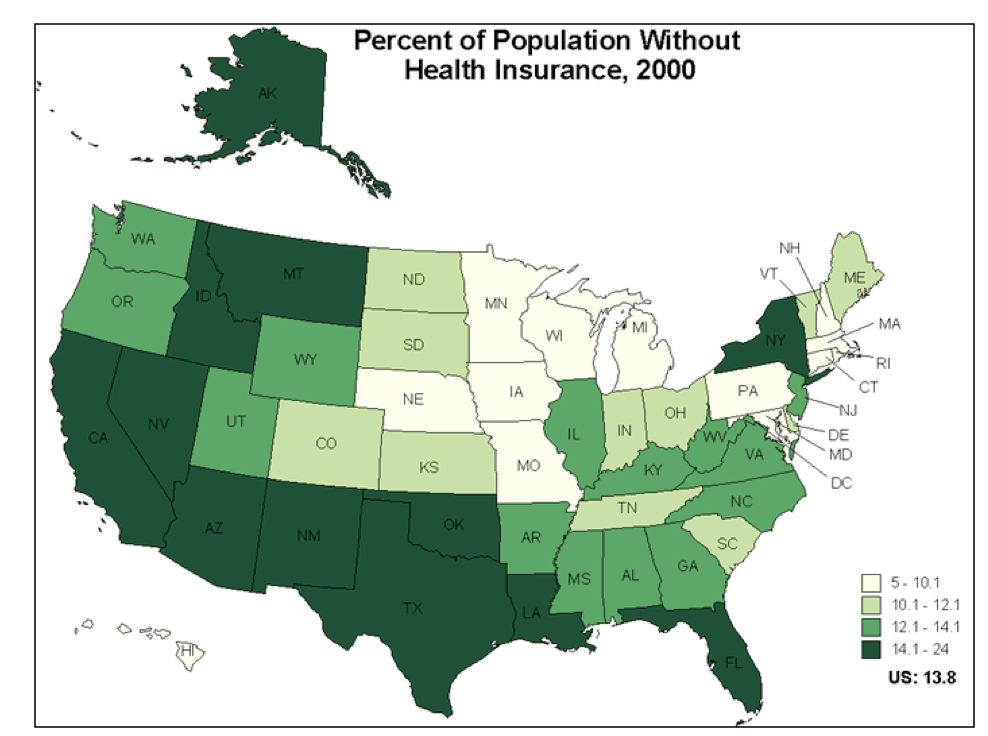
\includegraphics[width=0.6\linewidth]{image/colorblind4}
\end{frame}

%\begin{frame}
%\frametitle{Our color vision is limited...}
%Use distinctive colors when possible.
%\vfill
%\centering
%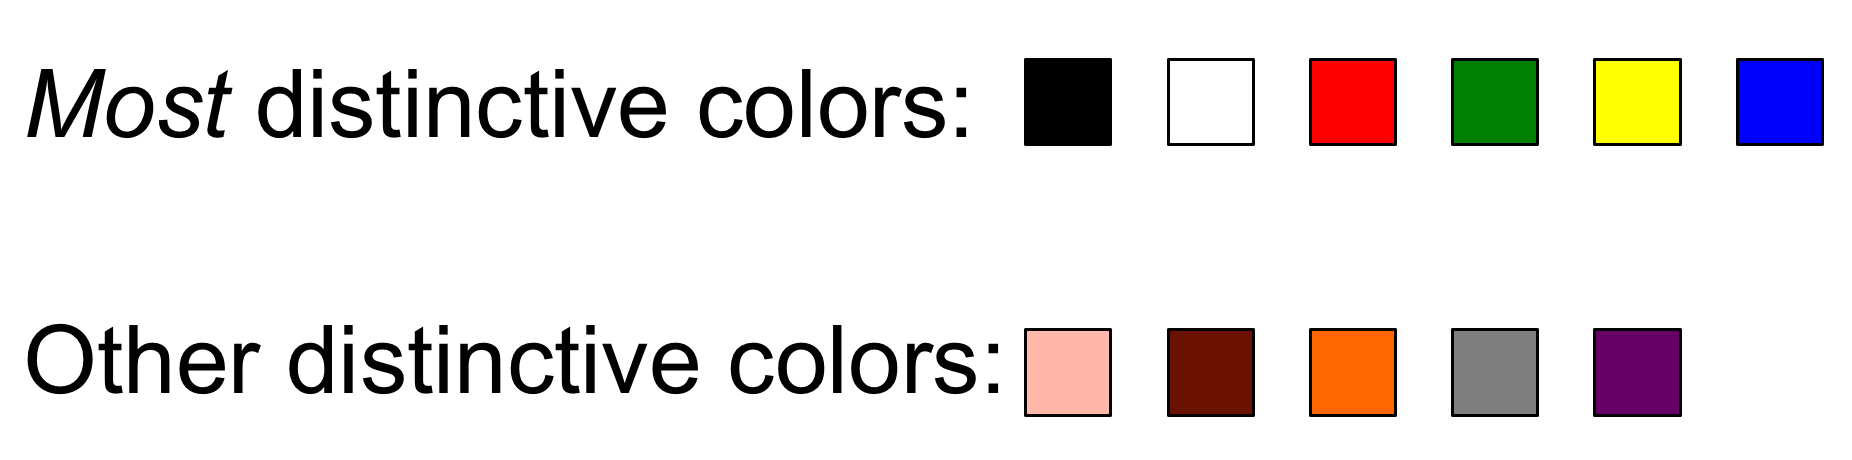
\includegraphics[width=0.8\linewidth]{image/colorblind6}
%\end{frame}

%\begin{frame}
%\begin{center} 
%\usebeamerfont*{frametitle} \usebeamercolor[fg]{frametitle}  5-mins break 
%\end{center}
%\end{frame}

\begin{frame}
\frametitle{Our peripheral vision is poor...}
Our view of vision is actually narrow...
\vfill
\centering
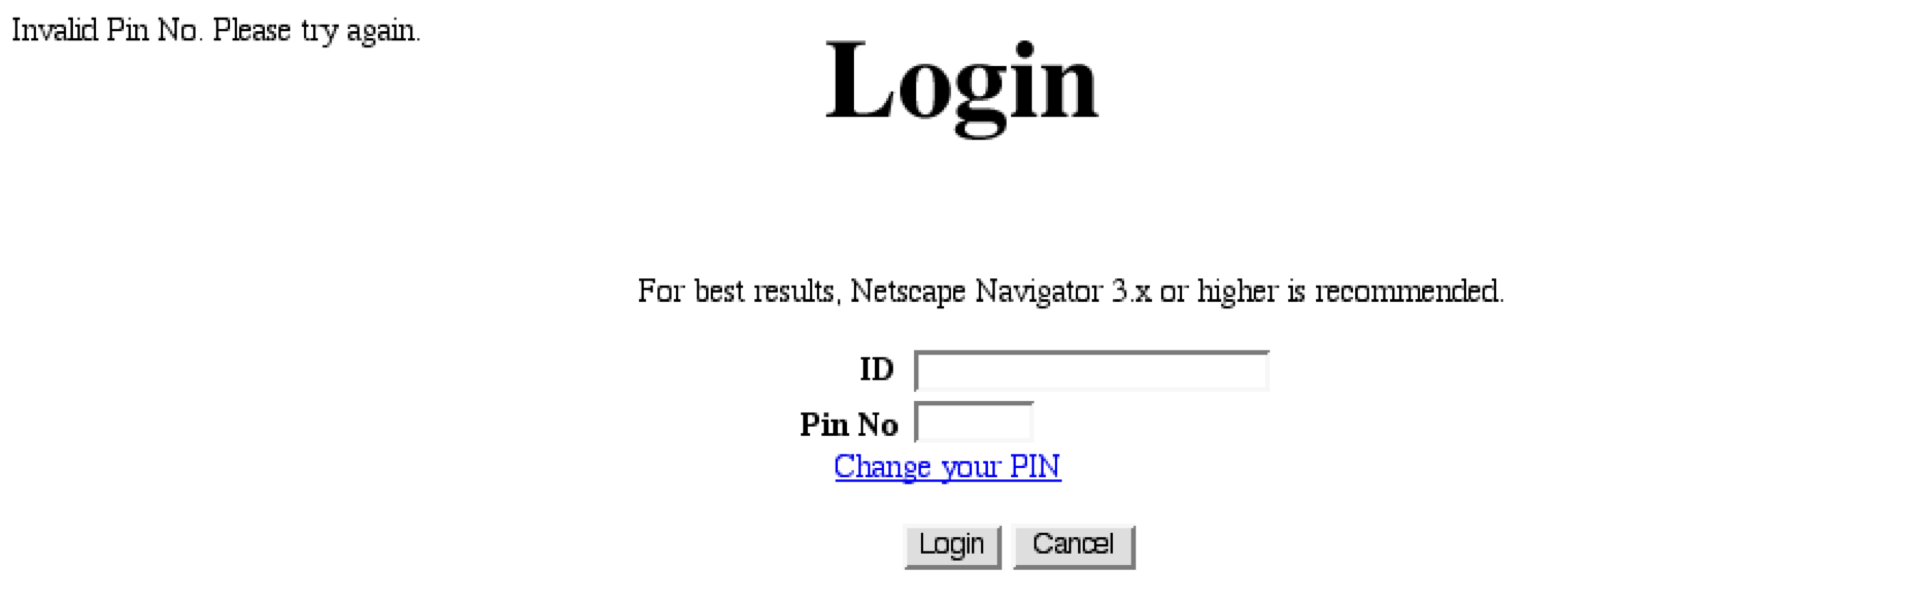
\includegraphics[width=1\linewidth]{image/peripheral}
\end{frame}

%\begin{frame}
%\frametitle{Our peripheral vision is poor...}
%Pixels are much denser in the center...
%\vfill
%\centering
%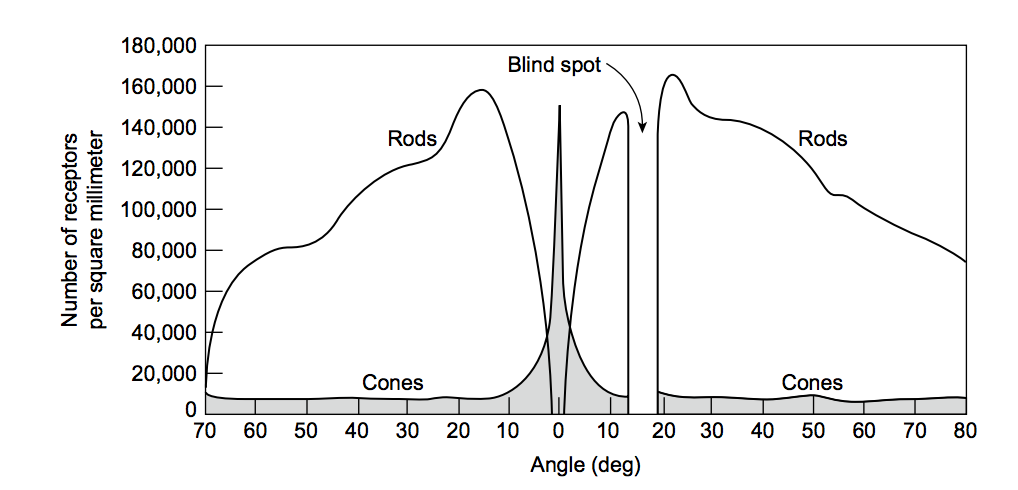
\includegraphics[width=1\linewidth]{image/peripheral2}
%\end{frame}

%\begin{frame}
%\frametitle{Our peripheral vision is poor...}
%Our eye resolution on the center is very high...higher than any of existing cameras
%\vfill
%\centering
%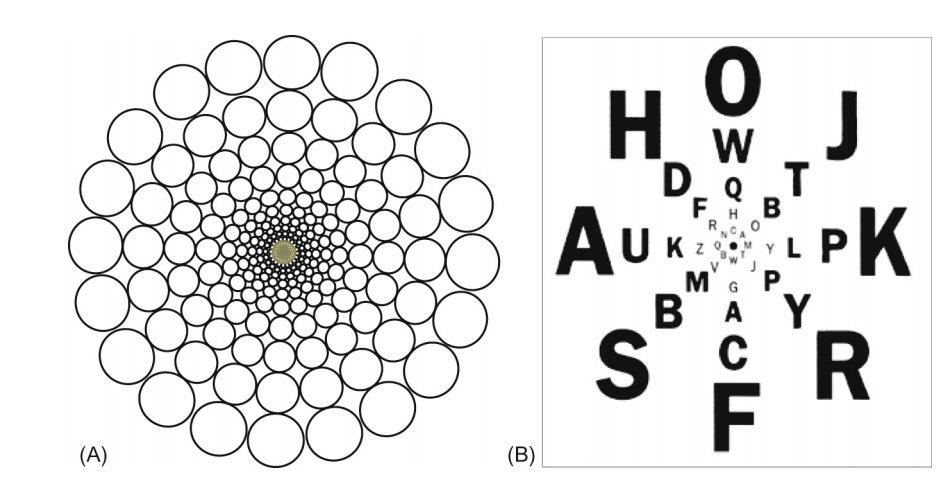
\includegraphics[width=1\linewidth]{image/peripheral3}
%\end{frame}

%\begin{frame}
%\frametitle{Our peripheral vision is poor...}
%Bad design...
%\vfill
%\centering
%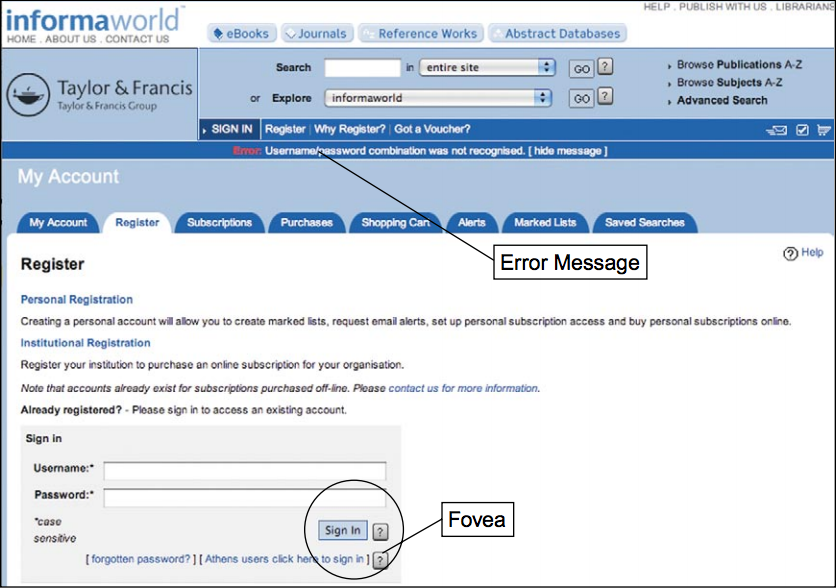
\includegraphics[width=1\linewidth]{image/peripheral4}
%\end{frame}

\begin{frame}
\frametitle{Our peripheral vision is poor...}
Bad design...
\vfill
\centering
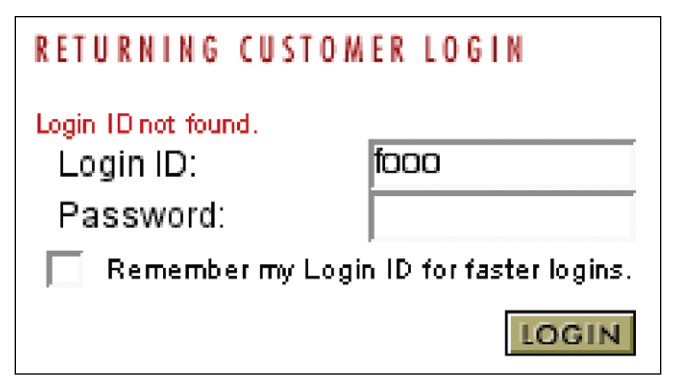
\includegraphics[width=1\linewidth]{image/peripheral5}
\end{frame}

\begin{frame}
\frametitle{Our peripheral vision is poor...}
Simulating the fovea...
\vfill
\centering
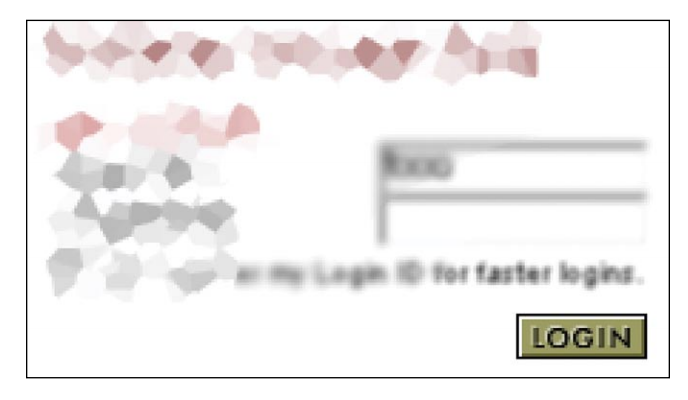
\includegraphics[width=0.8\linewidth]{image/peripheral6}
\end{frame}

\begin{frame}
\frametitle{Our peripheral vision is poor...}
Better design...
\vfill
\centering
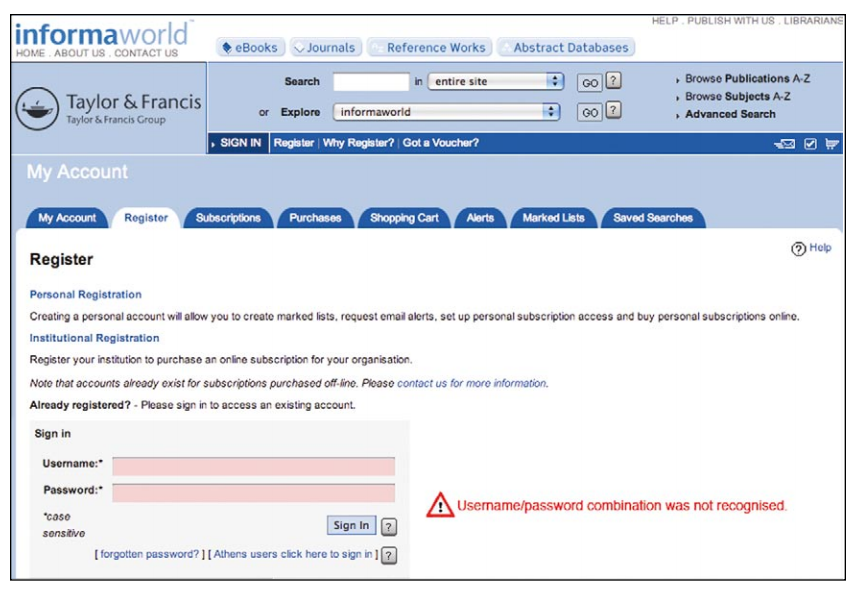
\includegraphics[width=0.8\linewidth]{image/peripheral7}
\end{frame}

\begin{frame}
\frametitle{Our peripheral vision is poor...}
Better design...
\vfill
\centering
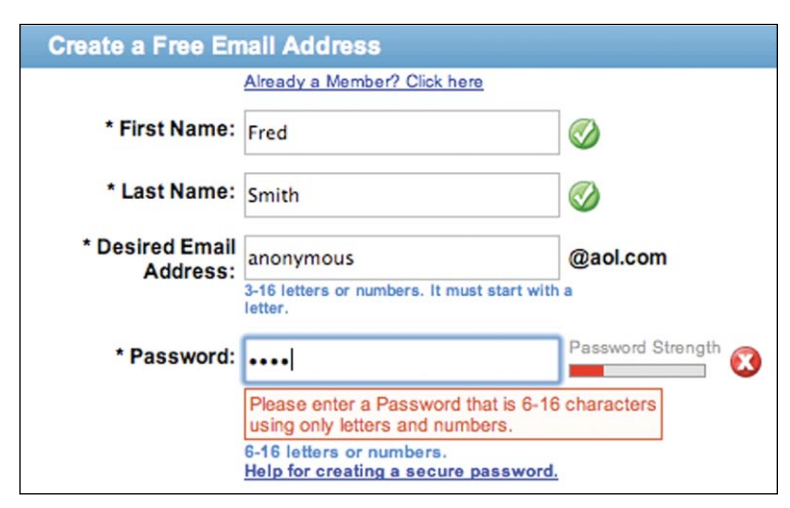
\includegraphics[width=0.8\linewidth]{image/peripheral8}
\end{frame}

%\begin{frame}
%\frametitle{Our peripheral vision is poor...}
%\begin{itemize}
%\item Put where users are looking
%\item Put near the errors
%\item Use red for errors
%\item Use error symbols
%\item Being redundant is good!!!
%\item Heavy design choices (Use sparingly!):
%\begin{itemize}
%\item Pop up dialogs
%\item Audio beep
%\item Flash and wiggle....
%\end{itemize}
%\end{itemize}
%\end{frame}

%\subsection{Visual search}
%
%\begin{frame}
%\frametitle{Visual search is linear...unless the target "pops"}
%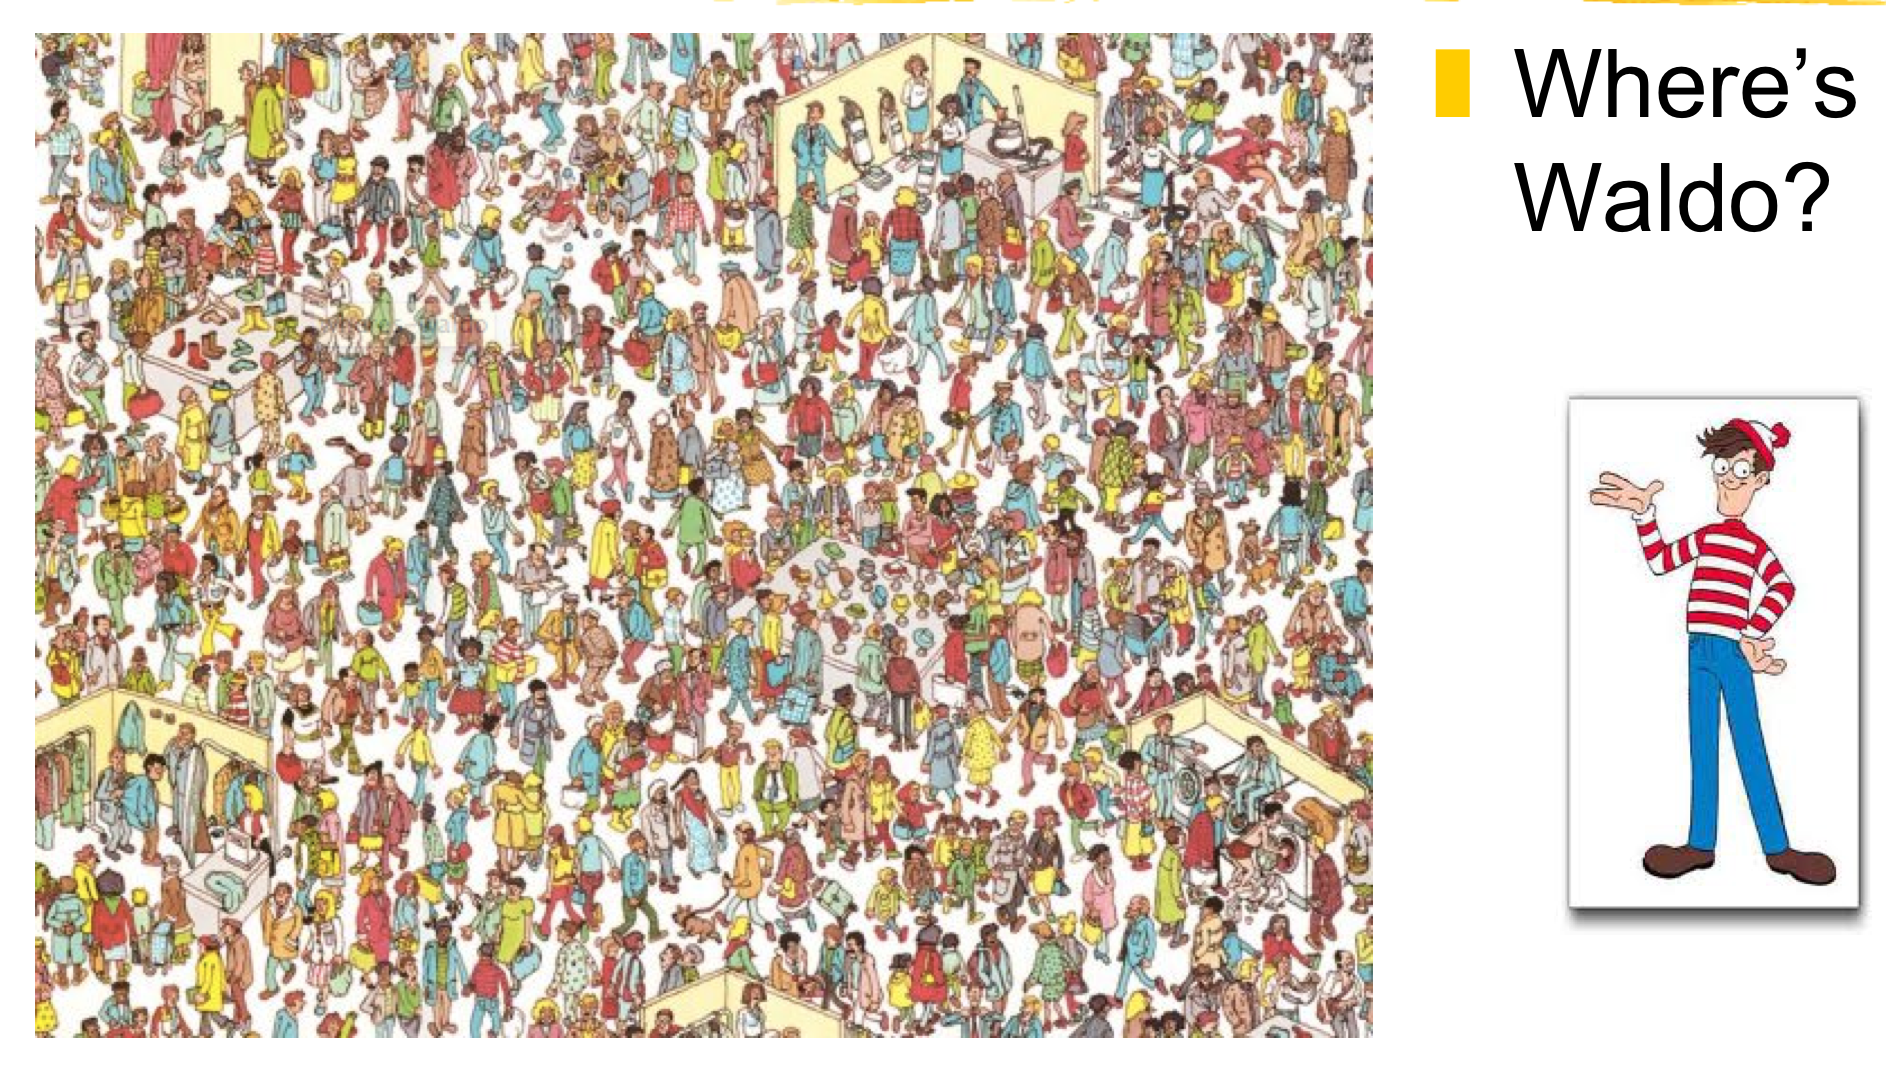
\includegraphics[width=1\linewidth]{image/search}
%\end{frame}
%
%\begin{frame}
%\frametitle{Visual search is linear...unless the target "pops"}
%\centering
%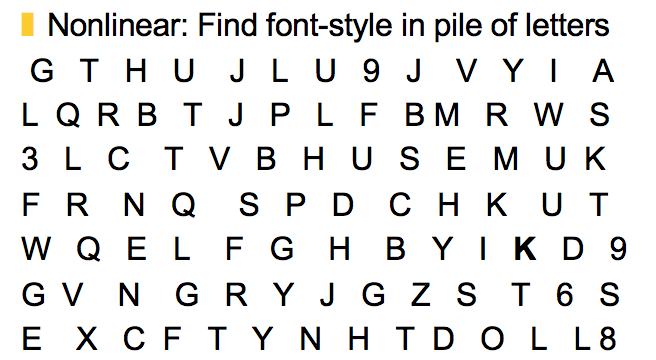
\includegraphics[width=0.8\linewidth]{image/search2}
%\end{frame}
%
%\begin{frame}
%\frametitle{Visual search is linear...unless the target "pops"}
%\centering
%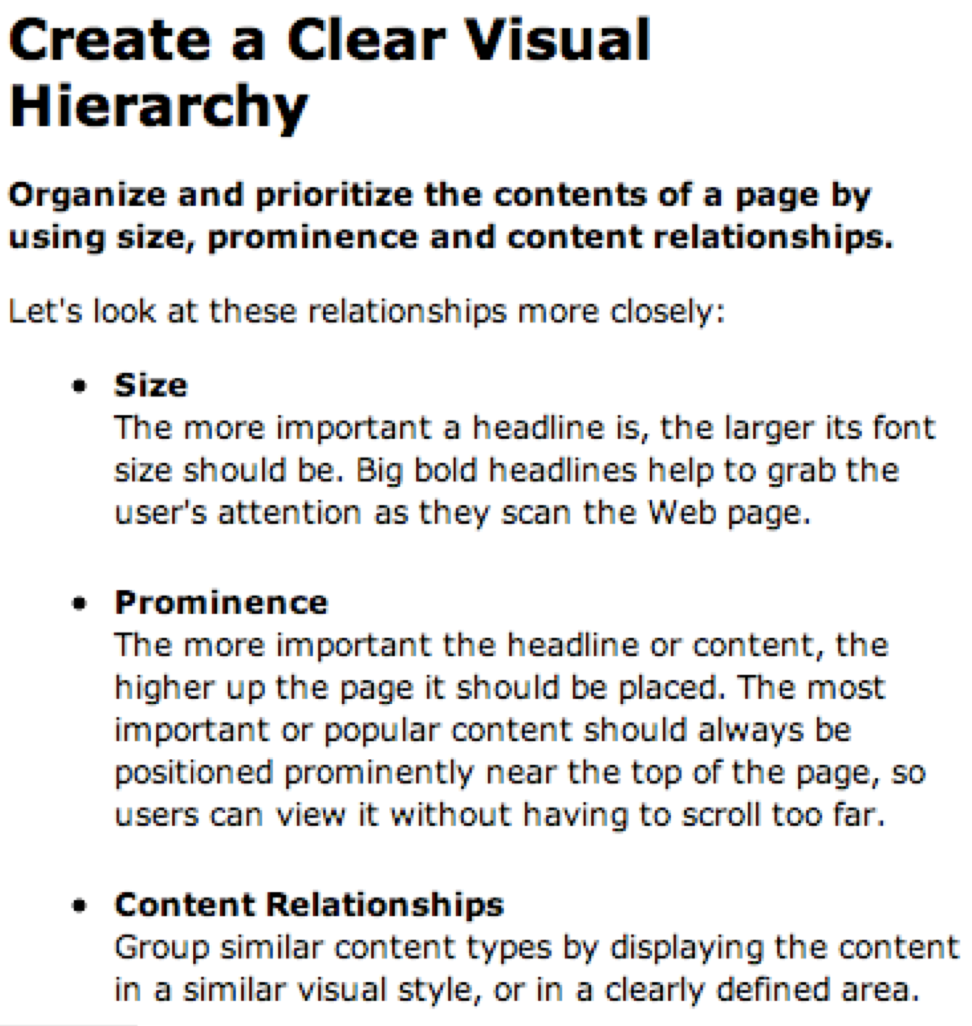
\includegraphics[width=0.5\linewidth]{image/search3}
%\end{frame}
%
%\begin{frame}
%\frametitle{Visual search is linear...unless the target "pops"}
%Icons help....arranging by alphabet also helps
%\centering
%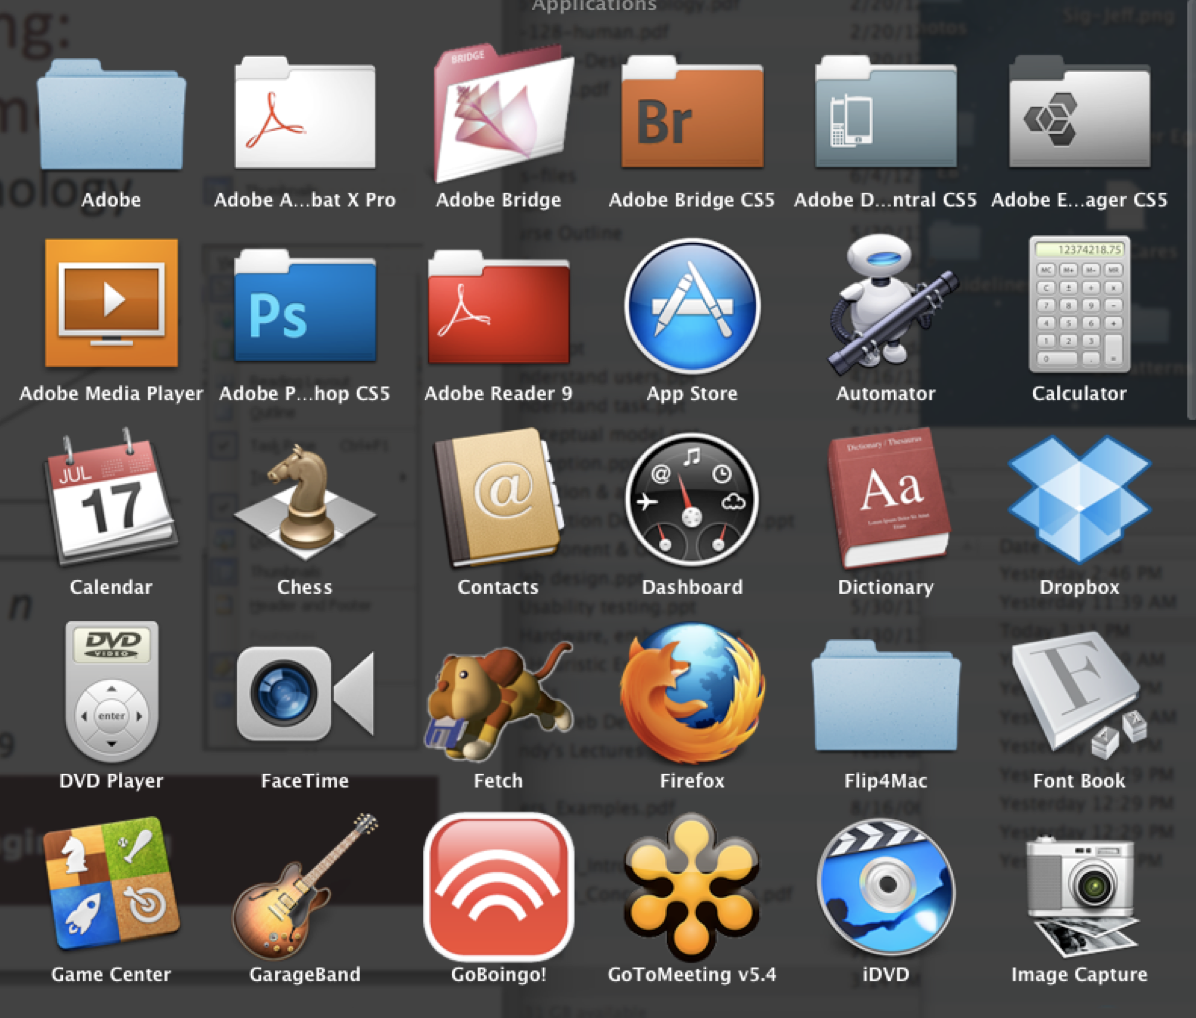
\includegraphics[width=0.6\linewidth]{image/search4}
%\end{frame}
%
%\begin{frame}
%\frametitle{Visual search is linear...unless the target "pops"}
%Visual search slows down by age...
%\centering 
%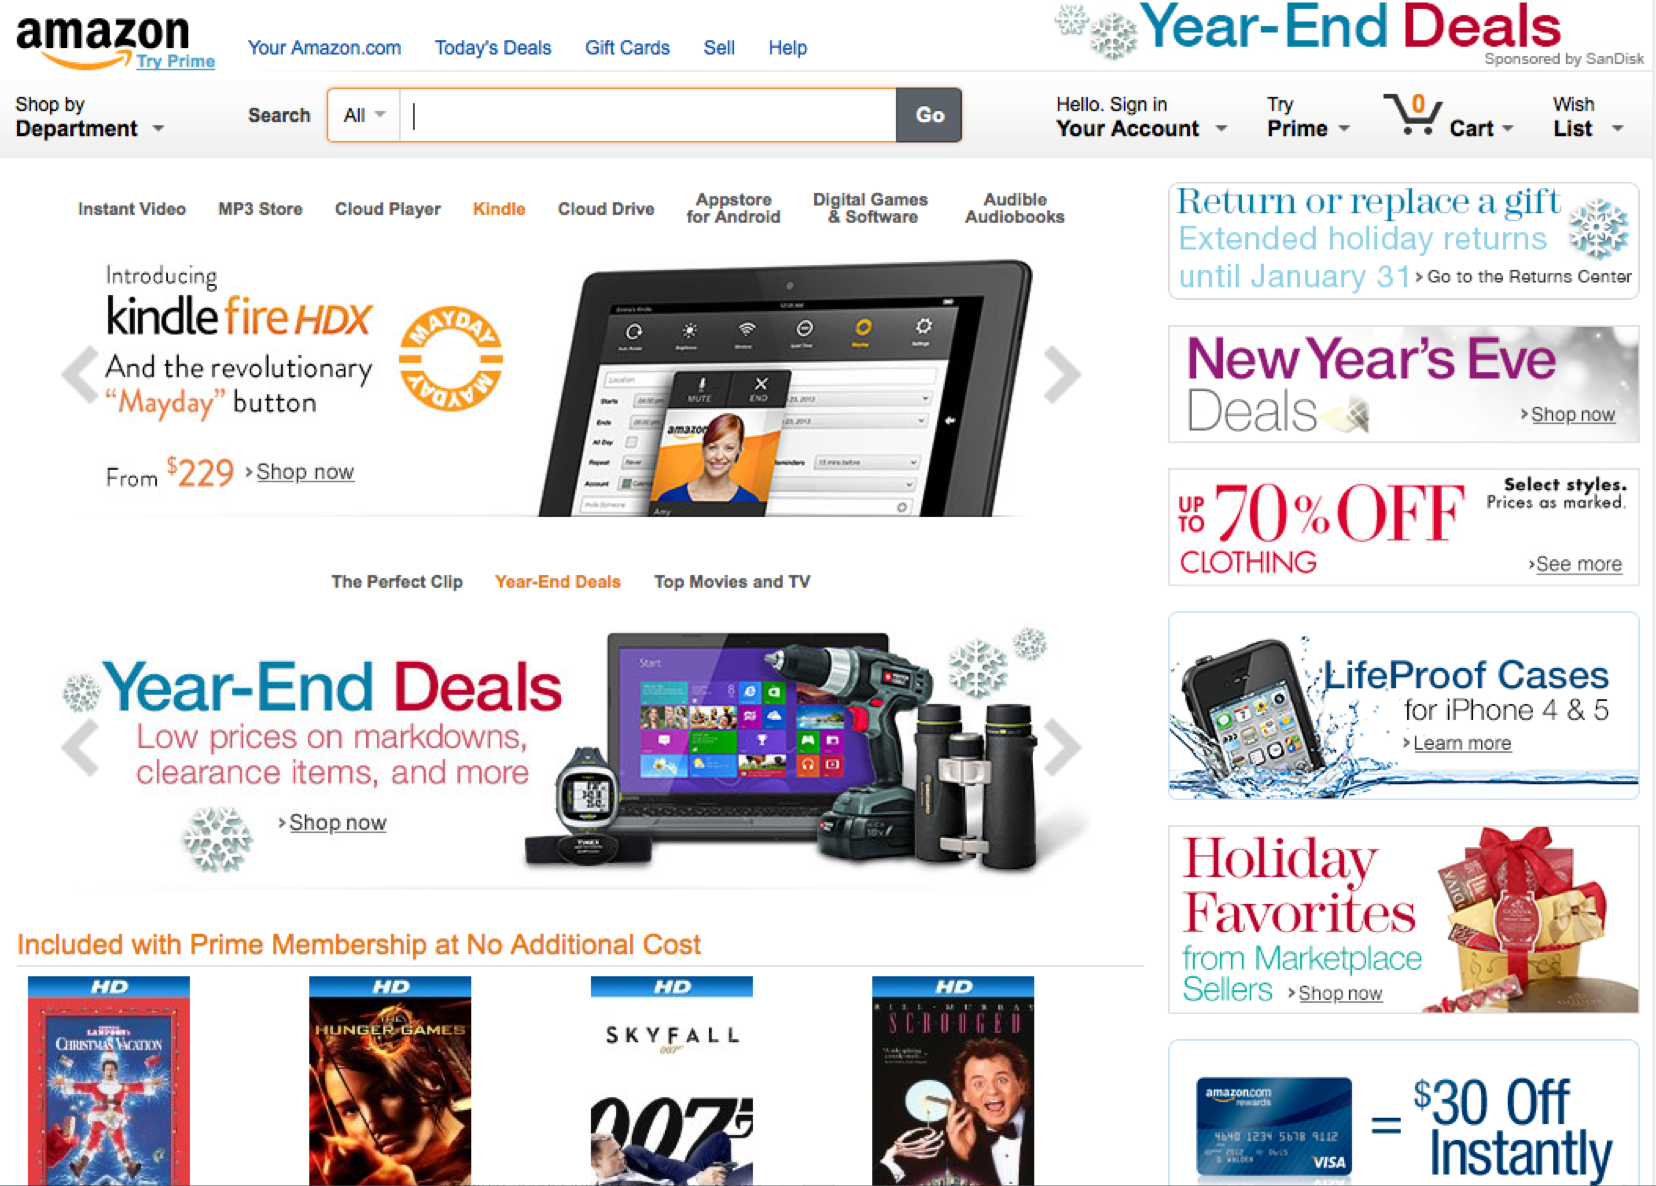
\includegraphics[width=0.7\linewidth]{image/search5}
%\end{frame}
%
%\begin{frame}
%	\frametitle{Talking about reading a bit}
%	\begin{itemize}
%		\item We're pre-wired for \textbf{language}
%		\item We are pre-wired for \textbf{pictures}
%		\item We are NOT pre-wired for \textbf{reading} - reading requires practice!
%		\item We \textbf{scan}, not look nor think $\rightarrow$ common mistakes on icon design
%	\end{itemize}
%\end{frame}

%\begin{frame}
%	\frametitle{Length helps reading}
%	\begin{figure}
%		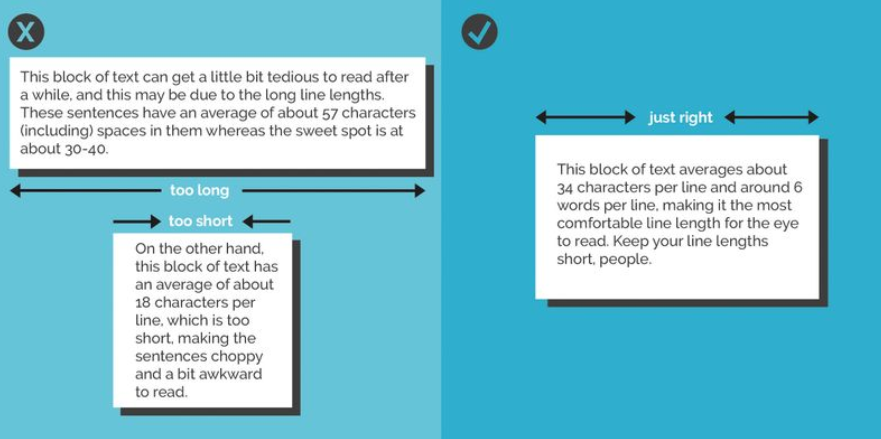
\includegraphics[width=0.9\linewidth]{image/length}
%	\end{figure}
%\end{frame}
%
%\begin{frame}
%	\frametitle{Space helps reading}
%	\begin{figure}
%		\includegraphics[width=0.9\linewidth]{image/space}
%	\end{figure}
%\end{frame}


%\begin{frame}
%	\frametitle{HCI and vision}
%	\begin{itemize}
%		\item Two important actions of eye: \textbf{fixation} and \textbf{saccades}
%		\item During fixation, eyes are stationary, typically last at least 200ms
%		\item Changing fixation requires a saccade - a rapid repositioning of the eyes
%		\item Saccades are quick, taking only 30 - 120ms
%		\begin{figure}
%			\includegraphics[width=0.6\linewidth]{image/eye}
%			\caption{Source: Fg 2.3 (Mackenzie)}
%		\end{figure}
%	\end{itemize}
%\end{frame}

\subsection{HCI and vision}

\begin{frame}
	\frametitle{HCI and vision}
	\begin{figure}
		\includegraphics[width=0.4\linewidth]{image/2-6}
		\caption{Source: Fg 2.6 (Mackenzie)}
	\end{figure}
\end{frame}

\begin{frame}
	\frametitle{HCI and vision}
	\begin{figure}
		\includegraphics[width=0.6\linewidth]{image/2-7}
		\caption{Source: Fg 2.7 (Mackenzie)}
	\end{figure}
\end{frame}

\begin{frame}
	\frametitle{HCI and vision}
	\begin{figure}
		\includegraphics[width=1\linewidth]{image/2-13}
		\caption{Source: Fg 2.13 (Mackenzie)}
	\end{figure}
\end{frame}

\subsection{Design implications}

\begin{frame}
\frametitle{Design implications}
	\begin{itemize}
		\item\textbf{Don't believe what users say}; instead understand their goals and knowledge (and what they don't know)
		\item Always exploit \textbf{structure} rules
		\item Use \textbf{color} very carefully
		\item Humans can focus only at \textbf{very tiny spot}.  Thus put where users are \textbf{looking}
		\item Use \textbf{affordance}, \textbf{convention}, \textbf{constraints}, \textbf{mapping} can increase visual search speed
	\end{itemize}
\end{frame}


%\begin{frame}
%	\frametitle{Reminders} % Table of contents slide, comment this block out to remove it
%	\begin{itemize}
%		\item Second draft due today - hard copy on shelf
%		\item HW10 due next Monday
%		\item Final draft due next Monday
%	\end{itemize}
%\end{frame}
%
%\begin{frame}
%\Huge{\centerline{Questions}}
%\end{frame}

%\begin{frame}
%\frametitle{Reminders} % Table of contents slide, comment this block out to remove it
%\begin{itemize}
%	\item \textbf{Project leaders} - Second paper reading summary due soon.  Hard copy on the shelf, and soft copy in Google classroom.
%\end{itemize}
%\end{frame}
%
%\begin{frame}
%\Huge{\centerline{CW/Project Questions}}
%\end{frame}

\section{Memory}

\begin{frame}
	\frametitle{Our memory is imperfect}
	\begin{itemize}
		\item Short Term Memory (STM or WM)
		\item Long Term Memory (LTM)
	\end{itemize}
	\centering
	\includegraphics[width=1\linewidth]{image/memory}
\end{frame}

\begin{frame}
	\frametitle{Our memory is imperfect}
	\centering
	\includegraphics[width=0.8\linewidth]{image/decay}
\end{frame}

\begin{frame}
	\frametitle{Short-term memory}
	\begin{itemize}
		\item Also known as working memory
		\item Can remember around 7 ($\pm$2) unrelated items (3-5 are better estimates, according to Jeff)
		\item Can stay for around $<$1 minute
		\item \textbf{Chunking} improves our short-term memory
	\end{itemize}
	\begin{figure}
		\includegraphics[width=0.6\linewidth]{image/2-18}
		\caption{Source: Figure 2.18 (Mackenzie): Digital lengths and memory}
	\end{figure}
\end{frame}

\begin{frame}
	\frametitle{Chunking}
	\begin{figure}
		\includegraphics[width=0.8\linewidth]{image/chunking}
	\end{figure}
\end{frame}

\begin{frame}
	\frametitle{Long-term memory}
	\begin{itemize}
		\item Stores life time experience but prone to error and biases
		\item Similar experience trigger same patterns $>$ \textbf{recognition}
		\item Internal neural activity triggers pattern $>$ \textbf{recall}
		\item Why we forget?
		\begin{itemize}
			\item \textbf{Decay theory}: proposes that memory fades due to mere passage of time - active rehearsing information is believed to counter this temporal decline
			\item \textbf{Interference theory}: proposes that similar information can make memories less accessible
		\end{itemize}
	\end{itemize}
\end{frame}

\begin{frame}
	\frametitle{Provide external memory aids}
	\centering
	\includegraphics[width=0.6\linewidth]{image/memory2}
\end{frame}

\begin{frame}
	\frametitle{Provide external memory aids}
	The use of flagging helps...
	\centering
	\includegraphics[width=1\linewidth]{image/memory3}
\end{frame}

\begin{frame}
	\frametitle{Provide external memory aids}
	History of commands helps...
	\centering
	\includegraphics[width=0.5\linewidth]{image/memory4}
\end{frame}

\begin{frame}
	\frametitle{Recognition much faster than recall}
	\begin{itemize}
		\item Use menus and metaphors
		\item Use auto-completion if recall is really needed
%		\item We assessed situations very quickly
%		\item We recognize faces fast
%		\item We recognize complex patterns
%		\item Command Line vs. Menus
%		\item Key guidelines: See and Choose are much preferable than Remember and Type
	\end{itemize}
	\centering
	\includegraphics[width=0.8\linewidth]{image/recognition}
\end{frame}

\subsection{Design implications}

\begin{frame}
	\frametitle{Design Implications}
		\begin{itemize}
			\item Use \textbf{convention} and \textbf{consistency}
			\item Use \textbf{recognition} instead of recall when possible (but do not forget ways for novice to transition to experts)
			\item Use \textbf{chunking} when possible; 3-5 rule
			\item \textbf{Put the knowledge in of the world} (Norman, 1988), e.g.,  bookmarks, history of commands, tagging, time stamping, reminders, marked emails, pwd etc.
		\end{itemize}
\end{frame}

%\begin{frame}
%	\frametitle{Context is important}
%	\begin{itemize}
%		\item When we memorize something, the context is automatically encoded
%		\item Sometimes it can be difficult for people to recall information that was encoded in a different context
%		\item “\textit{You are on a train and someone comes up to you and says hello. You don’t recognize him for a few moments but then realize it is one of your neighbors. You are only used to seeing your neighbor in the hallway of your apartment block and seeing ahim out of context makes him difficult to recognize initially}”
%	\end{itemize}
%\end{frame}

%\begin{frame}
	%\frametitle{Activities}
	%\begin{block}{Classwork}
		%Download latest PEBL from \url{http://pebl.sourceforge.net/download.html}
		
		%Perform Corsi experiment
		
		%Report your findings.  Submit your work on HW10
	%\end{block}
%\end{frame}


\section{Cognition}
	
\subsection{Attention}

\begin{frame}
\frametitle{Attention}
\begin{itemize}
\item Our attention is limited
\item Goldfish has an attention span of 9s, guess how much is of humans? 8s!  (In 2000, our attention span is 12s)
\item Do you remember what I discuss in the previous slide?  What did you eat yesterday morning?
\end{itemize}
	\begin{figure}
	\includegraphics[width=0.3\linewidth]{image/goldfish}
\end{figure}
\end{frame}

\begin{frame}
\frametitle{Our attention is on the goal, not the tools/person}
\centering
\url{https://www.youtube.com/watch?v=FWSxSQsspiQ}
\begin{figure}
\includegraphics[width=0.6\linewidth]{image/doorstudy}
\end{figure}
\end{frame}

%\begin{frame}
%	\frametitle{Consider "viewport" - bad example}
%	\begin{figure}
%		\includegraphics[width=0.8\linewidth]{image/viewport1}
%	\end{figure}
%\end{frame}
%
%\begin{frame}
%	\frametitle{Consider "viewport" - good example}
%	\begin{figure}
%		\includegraphics[width=0.75\linewidth]{image/viewport2}
%	\end{figure}
%\end{frame}
%
%\begin{frame}
%	\frametitle{Consider "hierarchy" - bad example}
%	\begin{figure}
%		\includegraphics[width=0.8\linewidth]{image/hierarchy}
%	\end{figure}
%\end{frame}

%\begin{frame}
%	\frametitle{Consider "hierarchy"}
%	\begin{figure}
%		\includegraphics[width=0.8\linewidth]{image/hierarchy2}
%	\end{figure}
%\end{frame}

%\begin{frame}
%	\frametitle{Consider "hierarchy" - good example}
%	\begin{figure}
%		\includegraphics[width=0.8\linewidth]{image/hierarchy3}
%	\end{figure}
%\end{frame}
%
%\begin{frame}
%	\frametitle{Use grid}
%	\begin{figure}
%		\includegraphics[width=0.8\linewidth]{image/grid}
%	\end{figure}
%\end{frame}
%
%\begin{frame}
%	\frametitle{Just enough for decisions - bad example}
%	\begin{figure}
%		\includegraphics[width=0.8\linewidth]{image/enough}
%	\end{figure}
%\end{frame}
%
%\begin{frame}
%	\frametitle{Just enough for decisions - good example}
%	\begin{figure}
%		\includegraphics[width=0.8\linewidth]{image/enough2}
%	\end{figure}
%\end{frame}
%
%\begin{frame}
%	\frametitle{One click theory}
%	Fewer scrolls, fewer hovers, fewer mouse moving, faster decision makings
%	\begin{figure}
%		\includegraphics[width=0.7\linewidth]{image/one-click}
%	\end{figure}
%\end{frame}

\begin{frame}
\frametitle{Loose ends}
\begin{itemize}
\item When we finish our goal, we often forget the "loose ends" of tasks
\begin{itemize}
\item Turning headlights of car off
\item Forgetting to take your ATM card after withdrawing money
\end{itemize}
\end{itemize}
	\begin{figure}
	\includegraphics[width=0.6\linewidth]{image/carlight}
\end{figure}
\end{frame}

\begin{frame}
	\frametitle{End with action}
	\begin{figure}
		\includegraphics[width=0.9\linewidth]{image/action}
	\end{figure}
\end{frame}

\begin{frame}
	\frametitle{Hearing capabilities}
	\begin{itemize}
		\item Human hearing begins with sounds of 0-10dB.  Conversational speech is about 50-70 dB.  Painful sound is about 120-140 dB
		\item Pitch is the frequency and human can perceive sounds in the range of 20Hz to 20,000Hz (mine was 200Hz!  How about yours?)
	\end{itemize}
	\centering
	\url{https://www.youtube.com/watch?v=qNf9nzvnd1k}
	\begin{figure}
		\includegraphics[width=0.6\linewidth]{image/soundf}
	\end{figure}
\end{frame}

\begin{frame}
	\frametitle{Multitasking}
	\begin{itemize}
		\item Humans cannot really multi-task, we can only quickly switch between multiple tasks in ms
	\end{itemize}
	\centering
	\url{https://www.youtube.com/watch?v=vJG698U2Mvo}
	\begin{figure}
		\includegraphics[width=0.6\linewidth]{image/gorilla}
	\end{figure}
\end{frame}

%\begin{frame}
%	\frametitle{Colors}
%	Color is \textbf{subjective}.  For example, do you believe in the following \textbf{color-emotion} mapping? 
%\end{frame}
%
%\begin{frame}
%	\frametitle{Colors}
%	Red - confidence, ambition.
%	\begin{figure}
%		\includegraphics[width=0.6\linewidth]{image/red}
%	\end{figure}
%\end{frame}
%
%\begin{frame}
%	\frametitle{Colors}
%	Yellow - youthfulness, creativity
%	\begin{figure}
%		\includegraphics[width=0.6\linewidth]{image/yellow}
%	\end{figure}
%\end{frame}
%
%\begin{frame}
%	\frametitle{Colors}
%	Green - nature, friendly
%	\begin{figure}
%		\includegraphics[width=0.6\linewidth]{image/green}
%	\end{figure}
%\end{frame}
%
%\begin{frame}
%	\frametitle{Colors}
%	Blue - trustworthiness, security, stability
%	\begin{figure}
%		\includegraphics[width=0.6\linewidth]{image/blue}
%	\end{figure}
%\end{frame}
%
%\begin{frame}
%	\frametitle{Colors}
%	Purple - luxury
%	\begin{figure}
%		\includegraphics[width=0.6\linewidth]{image/purple}
%	\end{figure}
%\end{frame}
%
%\begin{frame}
%	\frametitle{Colors}
%	Black - neutral
%	\begin{figure}
%		\includegraphics[width=0.6\linewidth]{image/black}
%	\end{figure}
%\end{frame}
%
%\begin{frame}
%	\frametitle{Colors}
%	White - clean, simplicity, modern
%	\begin{figure}
%		\includegraphics[width=0.6\linewidth]{image/white}
%	\end{figure}
%\end{frame}

%\begin{frame}
%	\frametitle{Color guidelines}
%	60-30-10 rule
%	\begin{itemize}
%		\item 60 main color - suits and pants
%		\item 30 accent color - shirt
%		\item 10 another accent color - tie
%	\end{itemize}
%	\begin{figure}
%		\includegraphics[width=0.8\linewidth]{image/60}
%	\end{figure}
%\end{frame}
%
%\begin{frame}
%	\frametitle{Color guidelines}
%	Use tint and shades - HSB (HUE, Saturation, Brightness), opacity
%	\begin{figure}
%		\includegraphics[width=0.8\linewidth]{image/hsb}
%	\end{figure}
%\end{frame}

%\begin{frame}
%\begin{center} 
%\usebeamerfont*{frametitle} \usebeamercolor[fg]{frametitle}  5-mins break 
%\end{center}
%\end{frame}

\subsection{Learning}

\begin{frame}
	\frametitle{Learning}
	\begin{itemize}
			\item \textbf{Convention} helps learning
			\item \textbf{Feedback} helps learning
			\item \textbf{Risk} is low
			\item \textbf{Reward} is high
		\end{itemize}
\end{frame}

%\begin{frame}
%	\frametitle{Geek-speak hurts learning}
%	\begin{figure}
%		\includegraphics[width=1\linewidth]{image/geek}
%	\end{figure}
%\end{frame}

%\begin{frame}
%	\frametitle{Geek-speak hurts learning}
%	\begin{figure}
%		\includegraphics[width=1\linewidth]{image/geek2}
%	\end{figure}
%\end{frame}
%
%\begin{frame}
%	\frametitle{Geek-speak hurts learning}
%	\begin{figure}
%		\includegraphics[width=0.8\linewidth]{image/geek3}
%	\end{figure}
%\end{frame}
%
%\begin{frame}
%	\frametitle{Familiar term helps learning}
%	\begin{figure}
%		\includegraphics[width=0.7\linewidth]{image/familiar}
%	\end{figure}
%\end{frame}


\begin{frame}
	\frametitle{Convention helps learning}
	Always preach...follows convention!
	\centering
	\includegraphics[width=0.8\linewidth]{image/footer}
\end{frame}

\begin{frame}
	\frametitle{Convention helps learning}
	Always preach...follows convention!
	\centering
	\includegraphics[width=0.8\linewidth]{image/navbar}
\end{frame}

\begin{frame}
	\frametitle{Convention helps learning}
	Convention is about "stealing" but make it better
	\centering
	\includegraphics[width=0.8\linewidth]{image/filter}
\end{frame}

\begin{frame}
	\frametitle{Feedback helps learning}
	Feedback informs us how to become better
	\centering
	\includegraphics[width=0.8\linewidth]{image/game2}
\end{frame}

\begin{frame}
	\frametitle{Risk is low}
	\begin{itemize}
		\item \textbf{Cheap failures} - no ways to make errors; easy to recover
	\end{itemize}
	\centering
	\includegraphics[width=0.5\linewidth]{image/playagain}
\end{frame}

\begin{frame}
	\frametitle{Rewards}
	\begin{itemize}
		\item If you decide to break the cycle and reinvent something new
		\begin{itemize}
			\item make sure its\textbf{ reward exceeds learning effort}
			\item make sure it's \textbf{learnable} and  able to master over time!
			\item even better, \textbf{expert can still learn} something, i.e., novice vs. expert mode
		\end{itemize}
		\item \textbf{Games} are  fun, because everytime we play, \textbf{we get better, to no limits.}   (Self Determination Theory, 1985)
	\end{itemize}
	\centering
	\includegraphics[width=0.5\linewidth]{image/game}
\end{frame}

\subsection{Reasoning}

\begin{frame}
	\frametitle{System 1 and System 2}
	\begin{itemize}
		\item Our brain has two systems: system 1 and system 2
		\item \textbf{System 1} is the \textit{irrational} brain - fast, automatic, unconscious, yet govern most of our behavior
		\item \textbf{System 2} is the \textit{rational} brain - slow, precise, conscious, "believes" it governs our behaviors
	\end{itemize}
\end{frame}

\begin{frame}
	\frametitle{System 1 and 2}
	\centering
	\includegraphics[width=0.8\linewidth]{image/brain}
\end{frame}

\begin{frame}
	\frametitle{System 1 and System 2}
	\begin{itemize}
		\item A baseball and a bat together cost 110.  The bat costs 100 more than the ball.
		How much does the ball cost? 
		\item System 1 instant answer: 10  (wrong)
		\item System 2 may reject that answer.  Or not.
		\item System 2 can calculate correct answer; System 1 cannot.
	\end{itemize}
\end{frame}

\begin{frame}
	\frametitle{Human decisions are rarely rational}
	System 1 usually controls decisions but is very biased.
	\begin{itemize}
		\item \textbf{Losses} mean more than \textbf{gains}
		\item \textbf{Recent} history and strong memories "feel" more
		\item \textbf{Experience} and \textbf{intuition} means more than mountains of statistics and data
		\item People \textbf{avoid risks} for potential gains, but \textbf{take risks} for potential losses
		\item Influence by \textbf{word} (75\% survival rate vs. 25\% mortality rate)
	\end{itemize}
\end{frame}

\begin{frame}
	\frametitle{Human decisions are rarely rational}
	Kahneman and Tversky: Fourfold Pattern \vfill
	\centering
	\includegraphics[width=0.8\linewidth]{image/fourfold}
	\begin{itemize}
		\item TL - eye surgery with 95\% success but afraid of eye loss
		\item TR - desperate investment with 95\% failure but still do it
		\item BL - only 5\% chance to win \textbf{lottery} but still do it
		\item BR - only 5\% chance to lose, but get \textbf{insurance}
	\end{itemize}
\end{frame}

\begin{frame}
	\frametitle{Human decisions are rarely rational}
	\centering
	\includegraphics[width=1\linewidth]{image/brain6}
\end{frame}

\begin{frame}
	\frametitle{Human decisions are rarely rational}
	\centering
	\includegraphics[width=1\linewidth]{image/brain7}
\end{frame}

\subsection{Design implications}

\begin{frame}
	\frametitle{Design Implications}
	\begin{itemize}
			\item \textbf{Prioritize} your information.   People only have around a window of \textbf{5-8s}.
			\item Remind\textbf{ loose ends} - e.g., return to default mode, disconnect after inactivity, end with action, etc.
			\item \textbf{Convention} and \textbf{feedback} helps learning.
			\item If it is something \textbf{new}, make sure learning is fun with l\textbf{ow risk }and \textbf{high rewards}.
			\item Don't assume people \textbf{will think or read or learn}.  We are irrational.
			\item Test regularly and quantitatively.   Don't only take \textbf{average} performance but take note of the \textbf{special} cases.
	\end{itemize}
\end{frame}

%
%\begin{frame}
%	\frametitle{Activities}
%	\begin{block}{Classwork}
%		- Download ReactionTimeExperiment.jar from \url{http://www.yorku.ca/mack/ExperimentSoftware/}.  
%		
%		- Perform experiment for all five matchings (each with 10 trials). 
%		
%		- Attempt to think of \textbf{three} research questions,  \textbf{three} corresponding hypotheses, and perform \textbf{analysis}.  Finally make a \textbf{50} words conclusion for \textbf{each} question.
%
%%- How reaction rates differ on different matching?\\
%%- How are the reaction times when there is a match and when there is no
%%match? (Not including simple search because there is no notion of match and no
%%match in it).\\		
%		
%%		- Does people get better after practice? That is, can humans improve their raw visual skills by practicing?
%%		
%%		- Does users who press faster tend to make more errors? 
%%		
%%		- How does the differences in length affect error rates?  
%		\end{block}
%\end{frame}

\begin{frame}
	\frametitle{Activities}
	\footnotesize
	\begin{block}{Classwork}
	\begin{itemize}
	\item Download latest PEBL from \url{http://pebl.sourceforge.net/download.html}
	\item Perform the Muller-Lyer experiment 2 times.   Combine the two csv files into one and perform analysis using any tool,  e.g., Excel.
	\item Attempt to think of \textbf{three} research questions,  \textbf{three} corresponding hypotheses, and perform \textbf{analysis}.  Finally make a \textbf{50} words conclusion for \textbf{each} question.
	\end{itemize}
%		- Does people get better after practice? That is, can humans improve their raw visual skills by practicing?
%		
%		- Does users who press faster tend to make more errors? 
%		
%		- How does the differences in length affect error rates?  
		
The challenge is to think what are good scientific questions, and do proper analysis.  Make sure all graphs have standard bar errors.
		
	\end{block}
\end{frame}
%
%\begin{frame}
%	\frametitle{Activities}
%	\begin{block}{Classwork}
%	\begin{itemize}
%		\item In PEBL, select one task you are interested. 
%		\item Carry out the same analysis as previous classwork.
%		\item Make sure you perform enough times to perform analysis.
%	\end{itemize}
%	\end{block}
%\end{frame}

%

%
%\begin{frame}
%\frametitle{Human decisions are rarely rational}
%\centering
%\includegraphics[width=0.8\linewidth]{image/brain3}
%\end{frame}
%
%\begin{frame}
%\frametitle{Human decisions are rarely rational}
%\centering
%\includegraphics[width=1\linewidth]{image/brain4}
%\end{frame}
%
%\begin{frame}
%\frametitle{Human decisions are rarely rational}
%\centering
%\includegraphics[width=1\linewidth]{image/brain5}
%\end{frame}
%
%\subsection{Mental models}
%
%\subsection{Motor skills}
%

%\begin{frame}
%	\frametitle{Reminders}
%	\begin{itemize}
%		\item Next week  workshops, and discussion of midterm exam question
%		\item Next next week midterm exam.  Open book/internet.  Cover everything from start til today.
%	\end{itemize}
%\end{frame}

\begin{frame}
\frametitle{What's next}
In following week,  read my slide on \textbf{Test} and these complimentary resources:
	\begin{itemize}
		\item Mackenzie, Chapter 6, \textbf{Hypothesis Testing},  Human Computer Interaction: An Empirical Research Perspective, 1st ed. (2013) 
		\item Yatani, Advanced Topics in Human-Computer Interaction, \url{http://yatani.jp/teaching/doku.php?id=2016hci:start}
	\end{itemize}
Please also download \textbf{JASP} for our next next week workshop.
\end{frame}

%-----


%------------------------------------------------

%\begin{frame}
%\frametitle{Blocks of Highlighted Text}
%\begin{block}{Block 1}
%Lorem ipsum dolor sit amet, consectetur adipiscing elit. Integer lectus nisl, ultricies in feugiat rutrum, porttitor sit amet augue. Aliquam ut tortor mauris. Sed volutpat ante purus, quis accumsan dolor.
%\end{block}
%
%\begin{block}{Block 2}
%Pellentesque sed tellus purus. Class aptent taciti sociosqu ad litora torquent per conubia nostra, per inceptos himenaeos. Vestibulum quis magna at risus dictum tempor eu vitae velit.
%\end{block}
%
%\begin{block}{Block 3}
%Suspendisse tincidunt sagittis gravida. Curabitur condimentum, enim sed venenatis rutrum, ipsum neque consectetur orci, sed blandit justo nisi ac lacus.
%\end{block}
%\end{frame}

%------------------------------------------------

%\begin{frame}
%\frametitle{Multiple Columns}
%\begin{columns}[c] % The "c" option specifies centered vertical alignment while the "t" option is used for top vertical alignment
%
%\column{.45\textwidth} % Left column and width
%\textbf{Heading}
%\begin{enumerate}
%\item Statement
%\item Explanation
%\item Example
%\end{enumerate}
%
%\column{.5\textwidth} % Right column and width
%Lorem ipsum dolor sit amet, consectetur adipiscing elit. Integer lectus nisl, ultricies in feugiat rutrum, porttitor sit amet augue. Aliquam ut tortor mauris. Sed volutpat ante purus, quis accumsan dolor.
%
%\end{columns}
%\end{frame}

%------------------------------------------------
%\section{Second Section}
%%------------------------------------------------
%
%\begin{frame}
%\frametitle{Table}
%\begin{table}
%\begin{tabular}{l l l}
%\toprule
%\textbf{Treatments} & \textbf{Response 1} & \textbf{Response 2}\\
%\midrule
%Treatment 1 & 0.0003262 & 0.562 \\
%Treatment 2 & 0.0015681 & 0.910 \\
%Treatment 3 & 0.0009271 & 0.296 \\
%\bottomrule
%\end{tabular}
%\caption{Table caption}
%\end{table}
%\end{frame}

%------------------------------------------------

%\begin{frame}
%\frametitle{Theorem}
%\begin{theorem}[Mass--energy equivalence]
%$E = mc^2$
%\end{theorem}
%\end{frame}

%------------------------------------------------

%\begin{frame}[fragile] % Need to use the fragile option when verbatim is used in the slide
%\frametitle{Verbatim}
%\begin{example}[Theorem Slide Code]
%\begin{verbatim}
%\begin{frame}
%\frametitle{Theorem}
%\begin{theorem}[Mass--energy equivalence]
%$E = mc^2$
%\end{theorem}
%\end{frame}\end{verbatim}
%\end{example}
%\end{frame}

%------------------------------------------------

%\begin{frame}
%\frametitle{Figure}
%Uncomment the code on this slide to include your own image from the same directory as the template .TeX file.
%%\begin{figure}
%%\includegraphics[width=0.8\linewidth]{test}
%%\end{figure}
%\end{frame}

%------------------------------------------------

%\begin{frame}[fragile] % Need to use the fragile option when verbatim is used in the slide
%\frametitle{Citation}
%An example of the \verb|\cite| command to cite within the presentation:\\~
%
%This statement requires citation \cite{p1}.
%\end{frame}

%------------------------------------------------

%\begin{frame}
%\frametitle{References}
%\footnotesize{
%\begin{thebibliography}{99} % Beamer does not support BibTeX so references must be inserted manually as below
%\bibitem[Smith, 2012]{p1} John Smith (2012)
%\newblock Title of the publication
%\newblock \emph{Journal Name} 12(3), 45 -- 678.
%\end{thebibliography}
%}
%\end{frame}

%------------------------------------------------

\begin{frame}
\Huge{\centerline{Questions}}
\end{frame}

%----------------------------------------------------------------------------------------

\end{document} 
